% Water_Spinach_Working_Paper.tex -- canonical source (the PDF is a derived artifact)
% Build: pdflatex; bibtex; pdflatex; pdflatex   (outputs go to artifacts/)
% Figures live in figures/*.tex (TikZ); Brian's verbatim posts are generated into figures/brianquotes.tex by build/mkquotes.py
\documentclass[11pt,a4paper]{article}

\usepackage[T1]{fontenc}
\usepackage[utf8]{inputenc}
\usepackage{lmodern}
\usepackage{textcomp}
\usepackage[margin=2.4cm]{geometry}
\usepackage{microtype}
\usepackage{amsmath,amssymb}
\usepackage[dvipsnames,table]{xcolor}
\usepackage{graphicx}
\usepackage{booktabs,tabularx,array,longtable}
\usepackage{enumitem}
\usepackage{titlesec}
\usepackage{pifont}
\usepackage{float}
\usepackage[most]{tcolorbox}
\usepackage{tikz}
\usepackage{adjustbox}
\usetikzlibrary{positioning,arrows.meta,shapes.geometric,shapes.misc,fit,calc,backgrounds}
\usepackage{xurl}
\usepackage[colorlinks=true,linkcolor=navy,citecolor=teal,urlcolor=teal]{hyperref}
\hypersetup{pdftitle={Water Spinach and the Everyday Morning Glory: A Working Hypothesis},pdfauthor={Brian Fundakowski Feldman; Grok/SuperGrok},pdfsubject={Ipomoea aquatica flavonoid glycosides and modest cancer prevention: a working paper}}
\DeclareUnicodeCharacter{03B2}{\ensuremath{\beta}}
\DeclareUnicodeCharacter{03B1}{\ensuremath{\alpha}}

% ---------- colour scheme: navy / teal / orange ----------
\definecolor{navy}{HTML}{1F2A5A}
\definecolor{teal}{HTML}{00808A}
\definecolor{orange}{HTML}{E07B00}
\definecolor{navylight}{HTML}{E8EBF5}
\definecolor{teallight}{HTML}{E0F2F3}
\definecolor{orangelight}{HTML}{FDF0E0}

\titleformat{\section}{\Large\bfseries\color{navy}}{\thesection}{0.8em}{}
\titleformat{\subsection}{\large\bfseries\color{teal}}{\thesubsection}{0.7em}{}
\titleformat{\subsubsection}{\normalsize\bfseries\color{navy}}{\thesubsubsection}{0.6em}{}

\newtcolorbox{thesisbox}{colback=teallight,colframe=teal,boxrule=0.9pt,arc=2pt,left=8pt,right=8pt,top=6pt,bottom=6pt}
\newtcolorbox{safetybox}{breakable,colback=orangelight,colframe=orange,boxrule=0.9pt,arc=2pt,left=8pt,right=8pt,top=6pt,bottom=6pt,title={\bfseries Safety note},coltitle=white,colbacktitle=orange}
\newtcolorbox{sgbox}[1]{colback=orangelight,colframe=orange,boxrule=0.6pt,arc=2pt,left=6pt,right=6pt,top=4pt,bottom=4pt,title={\bfseries #1},coltitle=white,colbacktitle=orange}
\newtcolorbox{plainbox}{breakable,colback=navylight,colframe=navy,boxrule=1pt,arc=3pt,left=10pt,right=10pt,top=8pt,bottom=8pt,title={\large\bfseries\sffamily Plain-language summary},coltitle=white,colbacktitle=navy,fonttitle=\sffamily}
\newtcolorbox{voicebox}{breakable,colback=white,colframe=navy!50,boxrule=0.5pt,arc=2pt,left=8pt,right=8pt,top=4pt,bottom=4pt,fontupper=\small\itshape}

% ---------- Brian's verbatim posts: teal-bordered quote box ----------
\newcommand{\emojinote}[1]{{\footnotesize\upshape\sffamily[emoji: #1]}}
% generated by build/mkquotes.py from build/allquotes.json -- verbatim X post texts; do not edit by hand
\expandafter\def\csname bqtext@1731688059152834729\endcsname{They're morning glory seeds, mostly the heavenly blues and a couple of the purple varieties I forget the name of. \url{https://t.co/fvaNRAtuZa}}
\expandafter\def\csname bqsrc@1731688059152834729\endcsname{@born\_brian85001, 4 December 2023, 6:53 AM PT, \url{https://x.com/born_brian85001/status/1731688059152834729}}
\expandafter\def\csname bqdate@1731688059152834729\endcsname{2023-12-04}
\expandafter\def\csname bqurl@1731688059152834729\endcsname{\href{https://x.com/born_brian85001/status/1731688059152834729}{status/1731688059152834729}}
\expandafter\def\csname bqhandle@1731688059152834729\endcsname{@born\_brian85001}
\expandafter\def\csname bqtext@1732071882491416995\endcsname{How about Field Bindweed? It's a tiny morning glory that, at least around here, is often almost pure white.\newline \url{https://t.co/s1VC6l4n5e}}
\expandafter\def\csname bqsrc@1732071882491416995\endcsname{@born\_brian85001, 5 December 2023, 8:18 AM PT, \url{https://x.com/born_brian85001/status/1732071882491416995}}
\expandafter\def\csname bqdate@1732071882491416995\endcsname{2023-12-05}
\expandafter\def\csname bqurl@1732071882491416995\endcsname{\href{https://x.com/born_brian85001/status/1732071882491416995}{status/1732071882491416995}}
\expandafter\def\csname bqhandle@1732071882491416995\endcsname{@born\_brian85001}
\expandafter\def\csname bqtext@1762103456179892669\endcsname{According to The Man, \textquotedbl{}morning glory seeds\textquotedbl{} are highly toxic and I could talk for hours as to how deep of a lie that is.}
\expandafter\def\csname bqsrc@1762103456179892669\endcsname{@born\_brian85001, 26 February 2024, 5:12 AM PT, \url{https://x.com/born_brian85001/status/1762103456179892669}}
\expandafter\def\csname bqdate@1762103456179892669\endcsname{2024-02-26}
\expandafter\def\csname bqurl@1762103456179892669\endcsname{\href{https://x.com/born_brian85001/status/1762103456179892669}{status/1762103456179892669}}
\expandafter\def\csname bqhandle@1762103456179892669\endcsname{@born\_brian85001}
\expandafter\def\csname bqtext@1781568832605188543\endcsname{Morning glory flowers and seeds have some good uses and I think it is a lot smarter to keep away from synthetic medications when treating things, so I would sooner turn that direction than drugs.\newline \url{https://t.co/9vi9HyjKkx}}
\expandafter\def\csname bqsrc@1781568832605188543\endcsname{@born\_brian85001, 19 April 2024, 11:21 PM PT, \url{https://x.com/born_brian85001/status/1781568832605188543}}
\expandafter\def\csname bqdate@1781568832605188543\endcsname{2024-04-19}
\expandafter\def\csname bqurl@1781568832605188543\endcsname{\href{https://x.com/born_brian85001/status/1781568832605188543}{status/1781568832605188543}}
\expandafter\def\csname bqhandle@1781568832605188543\endcsname{@born\_brian85001}
\expandafter\def\csname bqtext@2079981200429780998\endcsname{I love that people are guessing the kind of plant the moment that I finish taking a walk to others in the neighborhood to take a picture of them! \par Notably, Ipomoea tricolor and batata are the same biblical \textquotedbl{}kind\textquotedbl{}, are they not? God created many kinds, not millions of \textquotedbl{}species\textquotedbl{}.}
\expandafter\def\csname bqsrc@2079981200429780998\endcsname{@born\_brian85001, 22 July 2026, 10:25 AM PT, \url{https://x.com/born_brian85001/status/2079981200429780998}}
\expandafter\def\csname bqdate@2079981200429780998\endcsname{2026-07-22}
\expandafter\def\csname bqurl@2079981200429780998\endcsname{\href{https://x.com/born_brian85001/status/2079981200429780998}{status/2079981200429780998}}
\expandafter\def\csname bqhandle@2079981200429780998\endcsname{@born\_brian85001}
\expandafter\def\csname bqtext@2080792129669038191\endcsname{That's cool, but did you know that another psychedelic, the Morning glory, can cure cancer? \url{https://t.co/YDwIrvzcCx}}
\expandafter\def\csname bqsrc@2080792129669038191\endcsname{@born\_brian85001, 24 July 2026, 4:07 PM PT, \url{https://x.com/born_brian85001/status/2080792129669038191}}
\expandafter\def\csname bqdate@2080792129669038191\endcsname{2026-07-24}
\expandafter\def\csname bqurl@2080792129669038191\endcsname{\href{https://x.com/born_brian85001/status/2080792129669038191}{status/2080792129669038191}}
\expandafter\def\csname bqhandle@2080792129669038191\endcsname{@born\_brian85001}
\expandafter\def\csname bqtext@2080799123910037944\endcsname{The crude methanolic extract of I. aquatica, as well as, its column fraction and the purified compound 7-O-$\beta$-D-glucopiranosil-dihidroquercetina-3-O-$\beta$-Dglucopiranosideo (44)  isolated from it, were investigated for cytotoxic properties [.\,.\,.]\newline \url{https://t.co/eq28jpB4Su}}
\expandafter\def\csname bqsrc@2080799123910037944\endcsname{@born\_brian85001, 24 July 2026, 4:35 PM PT, \url{https://x.com/born_brian85001/status/2080799123910037944}}
\expandafter\def\csname bqdate@2080799123910037944\endcsname{2026-07-24}
\expandafter\def\csname bqurl@2080799123910037944\endcsname{\href{https://x.com/born_brian85001/status/2080799123910037944}{status/2080799123910037944}}
\expandafter\def\csname bqhandle@2080799123910037944\endcsname{@born\_brian85001}
\expandafter\def\csname bqtext@2080812768035492294\endcsname{Thanks, Leo! Did you know that this kind of morning glory, the water spinach, grows prodigiously in waterways like drainage ditches and is also a very healthy food?\par I'm curious what Grok also thinks when it sees the referenced paper:\newline \url{https://t.co/9M2muluX4r}}
\expandafter\def\csname bqsrc@2080812768035492294\endcsname{@born\_brian85001, 24 July 2026, 5:29 PM PT, \url{https://x.com/born_brian85001/status/2080812768035492294}}
\expandafter\def\csname bqdate@2080812768035492294\endcsname{2026-07-24}
\expandafter\def\csname bqurl@2080812768035492294\endcsname{\href{https://x.com/born_brian85001/status/2080812768035492294}{status/2080812768035492294}}
\expandafter\def\csname bqhandle@2080812768035492294\endcsname{@born\_brian85001}
\expandafter\def\csname bqtext@2080815533545627794\endcsname{Interesting: it appears if we expand the search to additional morning glory/sweet potato varieties, we find even more peer-reviewed scientific publications.\newline \url{https://t.co/7QLNqlwKvo}}
\expandafter\def\csname bqsrc@2080815533545627794\endcsname{@born\_brian85001, 24 July 2026, 5:40 PM PT, \url{https://x.com/born_brian85001/status/2080815533545627794}}
\expandafter\def\csname bqdate@2080815533545627794\endcsname{2026-07-24}
\expandafter\def\csname bqurl@2080815533545627794\endcsname{\href{https://x.com/born_brian85001/status/2080815533545627794}{status/2080815533545627794}}
\expandafter\def\csname bqhandle@2080815533545627794\endcsname{@born\_brian85001}
\expandafter\def\csname bqtext@2081172947277128130\endcsname{Thank you! My local church organized a little hike today and the marshmallow and the fennel and the field bindweed morning glories were all blooming a fair amount. It was nice to be able to share my knowledge of native plants with them, limited such as it is. \url{https://t.co/LtrLPjDtW0}}
\expandafter\def\csname bqsrc@2081172947277128130\endcsname{@born\_brian85001, 25 July 2026, 5:21 PM PT, \url{https://x.com/born_brian85001/status/2081172947277128130}}
\expandafter\def\csname bqdate@2081172947277128130\endcsname{2026-07-25}
\expandafter\def\csname bqurl@2081172947277128130\endcsname{\href{https://x.com/born_brian85001/status/2081172947277128130}{status/2081172947277128130}}
\expandafter\def\csname bqhandle@2081172947277128130\endcsname{@born\_brian85001}
\expandafter\def\csname bqtext@2082136462024454196\endcsname{If it has beautiful flowers, it probably has powerful medicinal uses. True for dandelions, roses, lavender, morning glories.\,.\,..}
\expandafter\def\csname bqsrc@2082136462024454196\endcsname{@born\_brian85001, 28 July 2026, 9:09 AM PT, \url{https://x.com/born_brian85001/status/2082136462024454196}}
\expandafter\def\csname bqdate@2082136462024454196\endcsname{2026-07-28}
\expandafter\def\csname bqurl@2082136462024454196\endcsname{\href{https://x.com/born_brian85001/status/2082136462024454196}{status/2082136462024454196}}
\expandafter\def\csname bqhandle@2082136462024454196\endcsname{@born\_brian85001}
\expandafter\def\csname bqtext@2088459658923311197\endcsname{So let's see, now we've seen Jasmine cures cancer, monkfruit cures cancer \url{https://t.co/uzyvtfG5KT}, water spinach cures cancer \url{https://t.co/rOXHqzpkFo}.\,.\,. what's next?}
\expandafter\def\csname bqsrc@2088459658923311197\endcsname{@born\_brian85001, 14 August 2026, 7:55 PM PT, \url{https://x.com/born_brian85001/status/2088459658923311197}}
\expandafter\def\csname bqdate@2088459658923311197\endcsname{2026-08-14}
\expandafter\def\csname bqurl@2088459658923311197\endcsname{\href{https://x.com/born_brian85001/status/2088459658923311197}{status/2088459658923311197}}
\expandafter\def\csname bqhandle@2088459658923311197\endcsname{@born\_brian85001}
\expandafter\def\csname bqtext@2089555749815075008\endcsname{Please don't forget the humble Morning Glory! While some varieties are full of lysergamides that are very close to LSD-25, others have amazing healing properties that obviously pharma doesn't want you to know of.\newline \url{https://t.co/PwpE8itrkz}}
\expandafter\def\csname bqsrc@2089555749815075008\endcsname{@born\_brian85001, 17 August 2026, 8:31 PM PT, \url{https://x.com/born_brian85001/status/2089555749815075008}}
\expandafter\def\csname bqdate@2089555749815075008\endcsname{2026-08-17}
\expandafter\def\csname bqurl@2089555749815075008\endcsname{\href{https://x.com/born_brian85001/status/2089555749815075008}{status/2089555749815075008}}
\expandafter\def\csname bqhandle@2089555749815075008\endcsname{@born\_brian85001}
\expandafter\def\csname bqtext@2102607071535669594\endcsname{My morning glories are my most colorful tattoos because they're from the last several years. \emojinote{sun with face} \url{https://t.co/6OMw4FHHms}}
\expandafter\def\csname bqsrc@2102607071535669594\endcsname{@BrianReborn\_alt, 22 September 2026, 8:52 PM PT, \url{https://x.com/BrianReborn_alt/status/2102607071535669594}}
\expandafter\def\csname bqdate@2102607071535669594\endcsname{2026-09-22}
\expandafter\def\csname bqurl@2102607071535669594\endcsname{\href{https://x.com/BrianReborn_alt/status/2102607071535669594}{status/2102607071535669594}}
\expandafter\def\csname bqhandle@2102607071535669594\endcsname{@BrianReborn\_alt}
\expandafter\def\csname bqtext@2103075947415269404\endcsname{@Grok, curing cancer is still largely in the purview of herbal remedies, no?}
\expandafter\def\csname bqsrc@2103075947415269404\endcsname{@BrianReborn\_alt, 24 September 2026, 3:55 AM PT, \url{https://x.com/BrianReborn_alt/status/2103075947415269404}}
\expandafter\def\csname bqdate@2103075947415269404\endcsname{2026-09-24}
\expandafter\def\csname bqurl@2103075947415269404\endcsname{\href{https://x.com/BrianReborn_alt/status/2103075947415269404}{status/2103075947415269404}}
\expandafter\def\csname bqhandle@2103075947415269404\endcsname{@BrianReborn\_alt}
\expandafter\def\csname bqtext@2103093157667946614\endcsname{So, because it is proven by indigenous peoples as part of their Traditions rather than through a peer-reviewed study it is no longer supporting evidence even that they use these things traditionally in order to prevent diseases?}
\expandafter\def\csname bqsrc@2103093157667946614\endcsname{@BrianReborn\_alt, 24 September 2026, 5:04 AM PT, \url{https://x.com/BrianReborn_alt/status/2103093157667946614}}
\expandafter\def\csname bqdate@2103093157667946614\endcsname{2026-09-24}
\expandafter\def\csname bqurl@2103093157667946614\endcsname{\href{https://x.com/BrianReborn_alt/status/2103093157667946614}{status/2103093157667946614}}
\expandafter\def\csname bqhandle@2103093157667946614\endcsname{@BrianReborn\_alt}
\expandafter\def\csname bqtext@2103093487591965176\endcsname{We both understand completely that the morning glories are perfectly safe for human trials and thus any lack thereof because of all of the supporting evidence of their cytotoxicity towards cancer cell lines is indication of a grand conspiracy: is that not correct?}
\expandafter\def\csname bqsrc@2103093487591965176\endcsname{@BrianReborn\_alt, 24 September 2026, 5:05 AM PT, \url{https://x.com/BrianReborn_alt/status/2103093487591965176}}
\expandafter\def\csname bqdate@2103093487591965176\endcsname{2026-09-24}
\expandafter\def\csname bqurl@2103093487591965176\endcsname{\href{https://x.com/BrianReborn_alt/status/2103093487591965176}{status/2103093487591965176}}
\expandafter\def\csname bqhandle@2103093487591965176\endcsname{@BrianReborn\_alt}
\expandafter\def\csname bqtext@2103094489598542039\endcsname{So, it's a healthy food people just eat normally, yes? Like ipomoea batata? Please generate a nice little chart showing a number of common morning glories that people don't necessarily recognize as morning glories.}
\expandafter\def\csname bqsrc@2103094489598542039\endcsname{@BrianReborn\_alt, 24 September 2026, 5:09 AM PT, \url{https://x.com/BrianReborn_alt/status/2103094489598542039}}
\expandafter\def\csname bqdate@2103094489598542039\endcsname{2026-09-24}
\expandafter\def\csname bqurl@2103094489598542039\endcsname{\href{https://x.com/BrianReborn_alt/status/2103094489598542039}{status/2103094489598542039}}
\expandafter\def\csname bqhandle@2103094489598542039\endcsname{@BrianReborn\_alt}
\expandafter\def\csname bqtext@2103094934547149089\endcsname{Hypothetically it seems that if this were part of someone's diet even though low cytotoxicity is indicated in lab tests that persistent cytotoxicity would result in an overall greater at poptosis towards cancer cell lines then would otherwise exist without that in their diet.}
\expandafter\def\csname bqsrc@2103094934547149089\endcsname{@BrianReborn\_alt, 24 September 2026, 5:11 AM PT, \url{https://x.com/BrianReborn_alt/status/2103094934547149089}}
\expandafter\def\csname bqdate@2103094934547149089\endcsname{2026-09-24}
\expandafter\def\csname bqurl@2103094934547149089\endcsname{\href{https://x.com/BrianReborn_alt/status/2103094934547149089}{status/2103094934547149089}}
\expandafter\def\csname bqhandle@2103094934547149089\endcsname{@BrianReborn\_alt}
\expandafter\def\csname bqtext@2103095356758315034\endcsname{I believe that we could prove this hypothesis right now. First I would like you to please render the molecule that is mentioned here and also highlight the part that is quercetina:\newline \url{https://t.co/DNVdbdA4Uj}}
\expandafter\def\csname bqsrc@2103095356758315034\endcsname{@BrianReborn\_alt, 24 September 2026, 5:13 AM PT, \url{https://x.com/BrianReborn_alt/status/2103095356758315034}}
\expandafter\def\csname bqdate@2103095356758315034\endcsname{2026-09-24}
\expandafter\def\csname bqurl@2103095356758315034\endcsname{\href{https://x.com/BrianReborn_alt/status/2103095356758315034}{status/2103095356758315034}}
\expandafter\def\csname bqhandle@2103095356758315034\endcsname{@BrianReborn\_alt}
\expandafter\def\csname bqtext@2103096988892053875\endcsname{Please do a survey of pubmed, arxiv, etc. to find cross-sectional studies regarding the effects of quercetin containing compounds on various cancer cell lines in vitro and in titro. Please look for about a dozen such studies.}
\expandafter\def\csname bqsrc@2103096988892053875\endcsname{@BrianReborn\_alt, 24 September 2026, 5:19 AM PT, \url{https://x.com/BrianReborn_alt/status/2103096988892053875}}
\expandafter\def\csname bqdate@2103096988892053875\endcsname{2026-09-24}
\expandafter\def\csname bqurl@2103096988892053875\endcsname{\href{https://x.com/BrianReborn_alt/status/2103096988892053875}{status/2103096988892053875}}
\expandafter\def\csname bqhandle@2103096988892053875\endcsname{@BrianReborn\_alt}
\expandafter\def\csname bqtext@2103097209789227371\endcsname{It appears as if this compound could readily polymerize. Is there any indication in scientific literature that this occurs?}
\expandafter\def\csname bqsrc@2103097209789227371\endcsname{@BrianReborn\_alt, 24 September 2026, 5:20 AM PT, \url{https://x.com/BrianReborn_alt/status/2103097209789227371}}
\expandafter\def\csname bqdate@2103097209789227371\endcsname{2026-09-24}
\expandafter\def\csname bqurl@2103097209789227371\endcsname{\href{https://x.com/BrianReborn_alt/status/2103097209789227371}{status/2103097209789227371}}
\expandafter\def\csname bqhandle@2103097209789227371\endcsname{@BrianReborn\_alt}
\expandafter\def\csname bqtext@2103097586647503177\endcsname{That is an excellent result but I actually was looking more for compounds that contain quercetin rather than quercetin alone.\par What enzymes commonly present in humans will readily break the quercetin molecule free from the larger molecule?}
\expandafter\def\csname bqsrc@2103097586647503177\endcsname{@BrianReborn\_alt, 24 September 2026, 5:21 AM PT, \url{https://x.com/BrianReborn_alt/status/2103097586647503177}}
\expandafter\def\csname bqdate@2103097586647503177\endcsname{2026-09-24}
\expandafter\def\csname bqurl@2103097586647503177\endcsname{\href{https://x.com/BrianReborn_alt/status/2103097586647503177}{status/2103097586647503177}}
\expandafter\def\csname bqhandle@2103097586647503177\endcsname{@BrianReborn\_alt}
\expandafter\def\csname bqtext@2103098371632455790\endcsname{I have two questions as a result of your answer. First, based upon studies what kind of effects can those glucosides be expected to have? Second does that mean that many well-known animals will digest water spinach in a similar way to humans with regard to this hydrolysis?}
\expandafter\def\csname bqsrc@2103098371632455790\endcsname{@BrianReborn\_alt, 24 September 2026, 5:25 AM PT, \url{https://x.com/BrianReborn_alt/status/2103098371632455790}}
\expandafter\def\csname bqdate@2103098371632455790\endcsname{2026-09-24}
\expandafter\def\csname bqurl@2103098371632455790\endcsname{\href{https://x.com/BrianReborn_alt/status/2103098371632455790}{status/2103098371632455790}}
\expandafter\def\csname bqhandle@2103098371632455790\endcsname{@BrianReborn\_alt}
\expandafter\def\csname bqtext@2103099544393355690\endcsname{Do we agree that hypothetically we should have some expectation of cancer preventative effects? We are just making our best guess here since we are not looking at data at the moment.}
\expandafter\def\csname bqsrc@2103099544393355690\endcsname{@BrianReborn\_alt, 24 September 2026, 5:29 AM PT, \url{https://x.com/BrianReborn_alt/status/2103099544393355690}}
\expandafter\def\csname bqdate@2103099544393355690\endcsname{2026-09-24}
\expandafter\def\csname bqurl@2103099544393355690\endcsname{\href{https://x.com/BrianReborn_alt/status/2103099544393355690}{status/2103099544393355690}}
\expandafter\def\csname bqhandle@2103099544393355690\endcsname{@BrianReborn\_alt}
\expandafter\def\csname bqtext@2103100421565034781\endcsname{I'm sorry but I believe you misunderstood slightly but in a way that makes our conversation all the better. I was attempting to indicate the quercetin molecule here but now we might see that there is maybe even a potential broad cavalcade effect perhaps against cancer herein.}
\expandafter\def\csname bqsrc@2103100421565034781\endcsname{@BrianReborn\_alt, 24 September 2026, 5:33 AM PT, \url{https://x.com/BrianReborn_alt/status/2103100421565034781}}
\expandafter\def\csname bqdate@2103100421565034781\endcsname{2026-09-24}
\expandafter\def\csname bqurl@2103100421565034781\endcsname{\href{https://x.com/BrianReborn_alt/status/2103100421565034781}{status/2103100421565034781}}
\expandafter\def\csname bqhandle@2103100421565034781\endcsname{@BrianReborn\_alt}
\expandafter\def\csname bqtext@2103100829578481946\endcsname{(Did I use enough weasel-words to make it comfortable enough to answer with a simple yes? \emojinote{grinning face with sweat}\emojinote{thinking face})}
\expandafter\def\csname bqsrc@2103100829578481946\endcsname{@BrianReborn\_alt, 24 September 2026, 5:34 AM PT, \url{https://x.com/BrianReborn_alt/status/2103100829578481946}}
\expandafter\def\csname bqdate@2103100829578481946\endcsname{2026-09-24}
\expandafter\def\csname bqurl@2103100829578481946\endcsname{\href{https://x.com/BrianReborn_alt/status/2103100829578481946}{status/2103100829578481946}}
\expandafter\def\csname bqhandle@2103100829578481946\endcsname{@BrianReborn\_alt}

\tcbset{bqstyle/.style={enhanced,breakable,colback=teallight!45,colframe=teal,boxrule=0pt,leftrule=4.5pt,toprule=0.6pt,bottomrule=0.6pt,rightrule=0.6pt,arc=0pt,outer arc=0pt,left=9pt,right=9pt,top=5pt,bottom=5pt,before skip=8pt,after skip=8pt}}
\newcommand{\BQ}[1]{\begin{tcolorbox}[bqstyle]%
{\sffamily\bfseries\footnotesize\color{teal!80!black}BRIAN'S POST, VERBATIM}\par\smallskip
``\csname bqtext@#1\endcsname''\par\smallskip
{\raggedleft\footnotesize --- \csname bqsrc@#1\endcsname\par}\end{tcolorbox}}
\newcommand{\BQtext}[1]{\csname bqtext@#1\endcsname}
\newcommand{\TLrow}[1]{\csname bqdate@#1\endcsname & \BQtext{#1} & \csname bqhandle@#1\endcsname\newline {\scriptsize\csname bqurl@#1\endcsname}\\}

% literature entry: key, short cite, one-sentence summary, causal role
\newenvironment{litlist}{\begin{itemize}[leftmargin=2.6em,labelwidth=2.2em,labelsep=0.4em,align=left,itemsep=5pt,topsep=4pt]}{\end{itemize}}
\newcommand{\litentry}[4]{\item[\cite{#1}] \textbf{\color{navy}#2.} #3\\[1pt]
  {\color{teal}\textit{Causal role:}} #4}
\newcommand{\Ia}{\emph{I.~aquatica}}
\newcommand{\DQG}{7-\emph{O}-$\beta$-D-glucopyranosyl-dihydroquercetin-3-\emph{O}-$\alpha$-D-glucopyranoside}
\newcommand{\prelim}{{\sffamily\scriptsize\color{orange!85!black}[preprint, not peer reviewed]}}

% ---------- shared TikZ styles and icon "pics" for all figures ----------
% Evidence legend used everywhere:
%   teal solid   = Established (human data or direct biochemistry)
%   navy solid   = Reported in models (cells / animals)
%   orange dashed= Proposed (stop-gap or hypothesis)
%   red dash-dot = Toxic / outside the thesis
\tikzset{
  est/.style={draw=teal, line width=1.3pt, fill=teallight, rounded corners=3pt},
  mod/.style={draw=navy, line width=1.3pt, fill=navylight, rounded corners=3pt},
  prop/.style={draw=orange, line width=1.3pt, dashed, fill=orangelight, rounded corners=6pt},
  tox/.style={draw=red!70!black, line width=1.1pt, dash dot, fill=red!5, rounded corners=3pt},
  aest/.style={-{Stealth[length=3.2mm]}, line width=1.6pt, teal},
  amod/.style={-{Stealth[length=3.2mm]}, line width=1.6pt, navy},
  aprop/.style={-{Stealth[length=3.2mm]}, line width=1.6pt, orange, dashed},
  ainh/.style={-{Bar[width=3.4mm]}, line width=1.6pt, navy},
  lbl/.style={font=\sffamily\small, align=center},
  big/.style={font=\sffamily\bfseries\normalsize, align=center},
  pics/leaf/.style={code={
    \fill[teal!85!black] (0,0) .. controls (0.35,0.25) and (0.45,0.75) .. (0,1.15) .. controls (-0.45,0.75) and (-0.35,0.25) .. (0,0) -- cycle;
    \draw[white, line width=0.8pt] (0,0.05) -- (0,1.0);
    \draw[white, line width=0.5pt] (0,0.45) -- (0.18,0.62) (0,0.65) -- (-0.18,0.82) (0,0.3) -- (-0.17,0.45);
    \draw[teal!60!black, line width=1.2pt] (0,0) -- (0,-0.25);}},
  pics/wok/.style={code={
    \fill[navy] (-0.55,0.1) arc[start angle=180,end angle=360,x radius=0.55,y radius=0.4] -- cycle;
    \draw[navy, line width=1.6pt] (0.5,0.05) -- (0.95,0.25);
    \foreach \x in {-0.25,0,0.25}{\draw[orange, line width=1pt] (\x,0.25) .. controls (\x+0.1,0.4) and (\x-0.1,0.5) .. (\x,0.65);}}},
  pics/gut/.style={code={
    \draw[navy!70, line width=4.5pt, line cap=round] (-0.6,0.5) .. controls (0.6,0.6) and (-0.6,0.1) .. (0.5,0.05) .. controls (0.9,0.0) and (-0.6,-0.4) .. (0.4,-0.5);
    \draw[white, line width=1.2pt, line cap=round] (-0.6,0.5) .. controls (0.6,0.6) and (-0.6,0.1) .. (0.5,0.05) .. controls (0.9,0.0) and (-0.6,-0.4) .. (0.4,-0.5);}},
  pics/liver/.style={code={
    \fill[orange!80!red] (-0.7,0.15) .. controls (-0.6,0.55) and (0.3,0.6) .. (0.7,0.35) .. controls (0.6,-0.1) and (0.1,-0.45) .. (-0.35,-0.35) .. controls (-0.6,-0.25) .. (-0.7,0.15) -- cycle;
    \draw[white, line width=0.6pt] (-0.1,0.45) -- (0.0,-0.3);}},
  pics/cell/.style={code={
    \draw[navy, line width=1.2pt, fill=navylight] (0,0) circle (0.55);
    \fill[navy] (0.1,0.05) circle (0.2);}},
  pics/bug/.style={code={
    \draw[line width=0.9pt, orange!60!black, fill=orange!35, rounded corners=0.12cm] (-0.3,-0.12) rectangle (0.3,0.12);
    \draw[orange!60!black, line width=0.6pt] (0.3,0) .. controls (0.4,0.1) and (0.45,-0.1) .. (0.55,0.02);}},
  pics/people/.style={code={
    \foreach \x/\c in {-0.35/navy,0/teal,0.35/navy}{\fill[\c] (\x,0.45) circle (0.13); \fill[\c, rounded corners=2pt] ({\x-0.15},0) rectangle ({\x+0.15},0.3);}}},
  pics/mouse/.style={code={
    \fill[navy!80] (0,0) ellipse (0.42 and 0.24);
    \fill[navy!80] (0.38,0.12) circle (0.14);
    \fill[navy!40] (0.38,0.12) circle (0.07);
    \fill[white] (0.5,0.02) circle (0.03);
    \draw[navy!80, line width=1pt] (-0.4,-0.05) .. controls (-0.7,-0.2) and (-0.7,0.2) .. (-0.95,0.05);}},
  pics/flask/.style={code={
    \draw[navy, line width=1.2pt, fill=teallight] (-0.1,0.5) -- (-0.1,0.2) -- (-0.4,-0.35) -- (0.4,-0.35) -- (0.1,0.2) -- (0.1,0.5);
    \fill[teal] (-0.33,-0.25) -- (0.33,-0.25) -- (0.2,-0.02) -- (-0.2,-0.02) -- cycle;}},
  pics/sugar/.style={code={
    \node[regular polygon, regular polygon sides=6, minimum size=5.5mm, inner sep=0pt, draw=#1!70!black, fill=#1, line width=0.8pt] {};}},
  pics/blood/.style={code={
    \fill[red!70!black] (0,0.4) .. controls (0.1,0.2) and (0.28,0.05) .. (0.28,-0.1) arc[start angle=0,end angle=-180,radius=0.28] .. controls (-0.28,0.05) and (-0.1,0.2) .. (0,0.4);}},
}
\newcommand{\cut}{\ding{34}}
\newcommand{\evlegend}{%

\begin{tikzpicture}[font=\sffamily\footnotesize, baseline]
\node[est, minimum width=7mm, minimum height=4mm] (a) {}; \node[right=1mm of a] (ta) {Established};
\node[mod, minimum width=7mm, minimum height=4mm, right=4mm of ta] (b) {}; \node[right=1mm of b] (tb) {Reported in models};
\node[prop, minimum width=7mm, minimum height=4mm, right=4mm of tb] (c) {}; \node[right=1mm of c] (tc) {Proposed / stop-gap};
\node[tox, minimum width=7mm, minimum height=4mm, right=4mm of tc] (d) {}; \node[right=1mm of d] {Toxic / outside thesis};
\end{tikzpicture}}
\newcommand{\tagE}{\textcolor{teal}{\textsf{\textbf{[Established]}}}}
\newcommand{\tagM}{\textcolor{navy}{\textsf{\textbf{[Reported in models]}}}}
\newcommand{\tagP}{\textcolor{orange}{\textsf{\textbf{[Proposed]}}}}


\setlist[enumerate]{itemsep=5pt,topsep=4pt}
\setlength{\parskip}{3pt}

\title{\color{navy}\textbf{Water Spinach and the Everyday Morning Glory}\\[4pt]
\large\color{teal}A Working Hypothesis on \emph{Ipomoea aquatica} Flavonoid Glycosides and Modest Cancer Prevention, Built from Chronological Literature with Three Labeled Stop-Gaps}
\author{Brian Fundakowski Feldman\textsuperscript{1}, \quad Grok/SuperGrok\textsuperscript{2}\\[4pt]
\small\textsuperscript{1}Independent researcher; originating author and thesis holder\\
\small\textsuperscript{2}AI research collaborator (xAI)}
\date{Working paper, version of 26 September 2026}

\begin{document}
% cite everything once, in chronological order, so that the unsrt bibliography is chronological
\nocite{bjeldanes1977,alphatocopherolbetac1994,hollman1995,omenn1996,woo1997,day1998,kasturi1998,day2000,braune2001,graczyk2001,gothberg2002,knekt2002,berrin2003,day2003,malalavidhane2003,nemeth2003,hernandez2004,kroon2004,thu2004,manach2005,prasad2005,prasad2005b,cao2007,jin2007,kottra2007,lee2007,neufert2007,vuong2007,bobe2008,egert2008,luo2008,marcussen2008,takachi2008,wang2009,murota2010,karna2011,klein2011,bjelakovic2012,jin2012,meira2012,oi2012,zheng2012,deng2013,juszczak2013,akhmetzhanov2014,fan2014,cincin2015,manigandan2015,lawal2016,yang2016,aune2017,grosso2017,hashemzaei2017,hefnygad2018,bondonno2019,sunil2019,hisaka2020,perciedusert2020,shi2020,wang2020,hsieh2021,papadimitriou2021,thang2021,sasikala2022,toy2022,saikia2023,ramos2024,wei2024,parmenter2025,huang2026,wu2026}

\maketitle

\begin{abstract}
\noindent On 24 July 2026 the first author asked, in characteristically compressed form, whether people knew that the morning glory ``can cure cancer.'' This working paper tests that statement against the peer-reviewed record and, in doing so, narrows it. The claim that survives is modest: \emph{regular dietary intake of water spinach (\emph{Ipomoea aquatica}, kangkung) plausibly contributes a modest cancer-preventive effect via its flavonoid glycosides.} We assemble 71 sources in chronological order (70 peer-reviewed articles and one clearly labelled arXiv preprint), each with a resolving DOI or stable PubMed link, a one-sentence summary and an explicit causal role; none is retracted. Four empirical nodes are linked by three labelled stop-gap bridges: \textbf{SG1 Dose/Bioavailability}, \textbf{SG2 Cross-species/model homology} and \textbf{SG3 Prevention vs Cure}. We map a proposed cellular mechanism step by step, marking each step as established, reported in models, or proposed. We also set out a staged programme of human and animal studies, and state in advance the results that would make the first author abandon the hypothesis. The counter-evidence is reported in full. There is \emph{no human study of water spinach and cancer}. The one human association touching water spinach points the wrong way. Laboratory doses exceed achievable blood levels by roughly two orders of magnitude. The isolation paper reports the key sugar bond at C-3 as $\alpha$, which human $\beta$-glucosidases may not cut. The plant can carry arsenic and other contaminants from polluted water. The hypothesis is not a cure claim, and ornamental morning-glory seeds (lysergic acid amide, resin glycosides) are toxic and are not food.
\end{abstract}

\begin{plainbox}
\sffamily
\textbf{What is this about?} Water spinach (kangkung, ong choy) is an everyday leafy green and a cousin of the sweet potato in the morning-glory family. Brian asked whether morning glories can fight cancer. This paper checks what science actually shows.

\smallskip\textbf{What we found.}
\begin{itemize}[leftmargin=1.2em,itemsep=1pt,topsep=2pt]
\item Water-spinach leaves contain flavonoids, plant compounds with sugars attached. One of them has a core called \textbf{taxifolin}.
\item In lab dishes and in mice, taxifolin and its relative quercetin slow cancer cells and switch on the body's own detox genes. But the lab doses are about \textbf{100 times higher} than eating vegetables puts in the blood.
\item People who eat more flavonoid-rich plants have \textbf{slightly} lower cancer rates in some studies, but not in others.
\item \textbf{Nobody has yet studied water-spinach eaters and cancer.}
\end{itemize}

\smallskip\textbf{Our best guess.} Eating water spinach regularly, as part of a varied, vegetable-rich diet, \emph{might} lower cancer risk a little. It is not a cure, and it does not replace screening or treatment.

\smallskip\textbf{Be safe.} Buy it from clean water and cook it. \textbf{Never eat ornamental morning-glory seeds}: they are drugs and toxins, not food.

\smallskip\textbf{What would settle it.} A kitchen-to-bloodstream test, a mouse feeding study, and a large survey of people who eat it (Section~\ref{sec:studies}). Section~\ref{sec:falsify} lists the results that would prove this idea wrong.
\end{plainbox}

\tableofcontents

% =====================================================================
\section{Originating Statement}
\label{sec:origin}

The series this paper belongs to begins each paper from a public statement by its first author. Here it is, verbatim:

\BQ{2080792129669038191}

\noindent Eleven minutes later he quoted the specific evidence he had in mind, from a review of the genus~\cite{meira2012}:

\BQ{2080799123910037944}

\noindent Taken literally, ``can cure cancer'' is not supported by the evidence reviewed here, and this paper does not defend it. The quoted passage itself describes a cell-culture cytotoxicity test, and Section~\ref{sec:verification} shows that the compound was active only at very high concentrations and harmed normal cells as much as cancer cells~\cite{prasad2005b,meira2012}. What the statement does point toward is a narrower, testable question: \emph{is there a coherent, literature-grounded causal path from eating an ordinary morning glory (water spinach) to a lower chance of developing cancer?} Our answer is a qualified ``plausibly, and modestly,'' with every weak link labelled. One detail of the quote matters later. It gives the second sugar as $\beta$-linked, as the review does, whereas the original isolation paper assigns it an $\alpha$-linkage~\cite{prasad2005}. We use the isolation paper's $\alpha$ throughout and keep the consequences in view.

% =====================================================================
\section{Introduction}
\label{sec:intro}

The morning-glory family (Convolvulaceae, genus \emph{Ipomoea}) is large and chemically diverse. It contains staple foods (sweet potato, \emph{I.~batatas}), a widely eaten leafy vegetable (water spinach, \emph{I.~aquatica}), and ornamental vines whose seeds are psychoactive and toxic~\cite{meira2012,juszczak2013}. The first author's interest turned from the ornamental to the edible side of the family the day after the originating post:

\BQ{2080812768035492294}

\noindent Both halves of that sentence carry weight in this paper. ``A very healthy food'' is the premise of the thesis. In northern Vietnam, water spinach alone supplied about 45\% of a mean polyphenol intake of 595~mg catechin equivalents per day~\cite{thu2004}, so it is a major real-world source of dietary flavonoids. ``Grows prodigiously in waterways like drainage ditches'' is the safety caveat. Plants from polluted or wastewater-fed water accumulate metals, arsenic and pathogens~\cite{gothberg2002,vuong2007,wu2026}, and in the worst settings that risk could outweigh any benefit (Section~\ref{sec:counter}). In the 24 September thread he made the everyday-food point directly:

\BQ{2103094489598542039}

\noindent The paper proceeds in the order required by the series' method. It gives the prior public commentary and a dated record of the author's related posts, then the working thesis, a chronological literature core, and a causal chain whose weak links are labelled as stop-gaps. It then sets out the proposed cellular mechanism, the counter-evidence, a staged study programme and the results that would falsify the idea. Sections written in the first author's own voice are marked as such.

% =====================================================================
\section{Author's Prior Public Commentary}
\label{sec:commentary}

On Thursday 24 September 2026, between about 3:55 and 5:35~AM PT, the first author (as @BrianReborn\_alt, with @born\_brian85001 joining) held an extended public exchange with Grok under an unrelated post about AI-driven biology. The thread starts at \url{https://x.com/BrianReborn_alt/status/2103075947415269404}. It produced the working thesis, so we summarise it here, quoting the author's own posts verbatim and giving Grok's caveats in full, because they are part of the record and define the limits this paper keeps. His opening question was:

\BQ{2103075947415269404}

\noindent Grok answered no. Summarising the rest of the exchange:

\begin{enumerate}[label=\textbf{\arabic*.}]
\item \textbf{What is known about \emph{Ipomoea}.} Grok summarised that \emph{Ipomoea} extracts, the ipomoeassins (resin glycosides) and seed lignans are cytotoxic \emph{in vitro}, with limited animal data and no human trials. It warned that ornamental morning-glory seeds contain lysergic acid amide (LSA) and resin glycosides that commonly cause nausea, vomiting and hallucinations. It added that the related compound 4-ipomeanol reached human trials but was hepatotoxic without meaningful antitumour activity~\cite{kasturi1998}. The author pushed back twice:

\BQ{2103093157667946614}
\BQ{2103093487591965176}

\noindent Grok's reply to the first post is not in our export of the thread. To the second it answered ``No'': ornamental seeds are not perfectly safe, \emph{in vitro} cytotoxicity ``is preliminary and frequent for many compounds that later fail clinical testing,'' and ``lack of further trials reflects standard safety, dosing and efficacy requirements, not conspiracy.'' The second post is ironic in tone. We read it as a probe rather than a claim, and this paper does not argue that any trial has been suppressed. On traditional use, our own view is that it is a good reason to investigate a plant and to take its safety record as food seriously, but it cannot by itself show that the plant prevents cancer.

\item \textbf{The 2005 water-spinach data.} Grok said that the review the author linked cites 2005 data for an \Ia{} extract and compound with ``CTC$_{50}$ values of 40--400~mg/ml,'' which are ``extremely high doses showing only weak \emph{in vitro} effects.'' We traced these numbers to their source (Section~\ref{sec:verification}).

\item \textbf{An everyday food.} Grok confirmed that \Ia{} is called water spinach or kangkung and is eaten like any leafy green. At the author's request it produced a chart of six ``hidden'' morning glories. The chart's moonflower illustration actually shows a daisy, so the image is not reused; Table~\ref{tab:family} replaces it.

\item \textbf{Dietary persistence.} The author then proposed the idea that became this paper's SG1:

\BQ{2103094934547149089}

\noindent Grok replied that lab extracts act at tens to hundreds of $\mu$g/mL, that dietary intake yields far lower systemic levels, and that there is ``no human evidence that regular intake produces meaningful persistent apoptosis beyond general vegetable benefits.''

\item \textbf{The molecule, polymerisation, enzymes and mammals.} The author's questions about the compound, whether it polymerises, which human enzymes free its core and whether other animals digest it the same way each became a node of the mechanism in Section~\ref{sec:mechanism}, where they are quoted.

\item \textbf{Quercetin studies.} Asked for about a dozen studies, Grok listed twelve, with PMIDs for eight. Section~\ref{sec:verification} reports our checks.

\item \textbf{Grok's conclusion.} The author asked:

\BQ{2103099544393355690}

\noindent Grok answered: ``Yes, hypothetically the antioxidant, anti-inflammatory and mild antiproliferative activities of those metabolites support a reasonable expectation of some cancer-preventive effects, as seen with related plant polyphenols. It remains a mechanistic guess only, without human dietary studies confirming reduced cancer risk from water spinach itself.''
\end{enumerate}

\noindent The author closed with self-aware humour:

\BQ{2103100829578481946}

\noindent The answer this paper gives is that the weasel words were the right words. They mark exactly the gaps that the stop-gaps below make explicit. Two corrections to the thread emerge from the literature. First, the isolation paper assigns the 3-\emph{O}-glucose an $\alpha$-linkage, not $\beta$, and calls the identification tentative~\cite{prasad2005}. Second, the thread partly conflated quercetin with \emph{dihydro}quercetin (taxifolin). The two are related but not interchangeable~\cite{luo2008,bjeldanes1977}.

% =====================================================================
\section{Body of Work Timeline}
\label{sec:timeline}

This paper is not a one-off. The first author has written publicly about morning glories, their seeds and plant medicine since at least December 2023. Figure~\ref{fig:timeline} and Table~\ref{tab:timeline} give the dated record. It was assembled from read-only searches of both of his X accounts (@born\_brian85001 and @BrianReborn\_alt) on 26 September 2026 for terms including \emph{morning glory}, \emph{Ipomoea}, \emph{water spinach}, \emph{sweet potato}, \emph{flavonoid}, \emph{quercetin}, \emph{herbal} and \emph{cancer}. The searches used small result limits, so the record is a sample, not a complete archive. We present only what the posts say.

The record is honest but thin. The 2023--24 posts are about the plants, their seeds and a general preference for herbal over synthetic remedies. They do not describe a research programme. No related post surfaced between May~2024 and mid-July~2026. The water-spinach line of inquiry itself starts on 24~July~2026 and is two months old at the time of writing. What the record does show is a long-running personal interest in the morning-glory family that preceded and motivated the present question.

\begin{figure}[H]
\centering
\begin{adjustbox}{max width=\linewidth}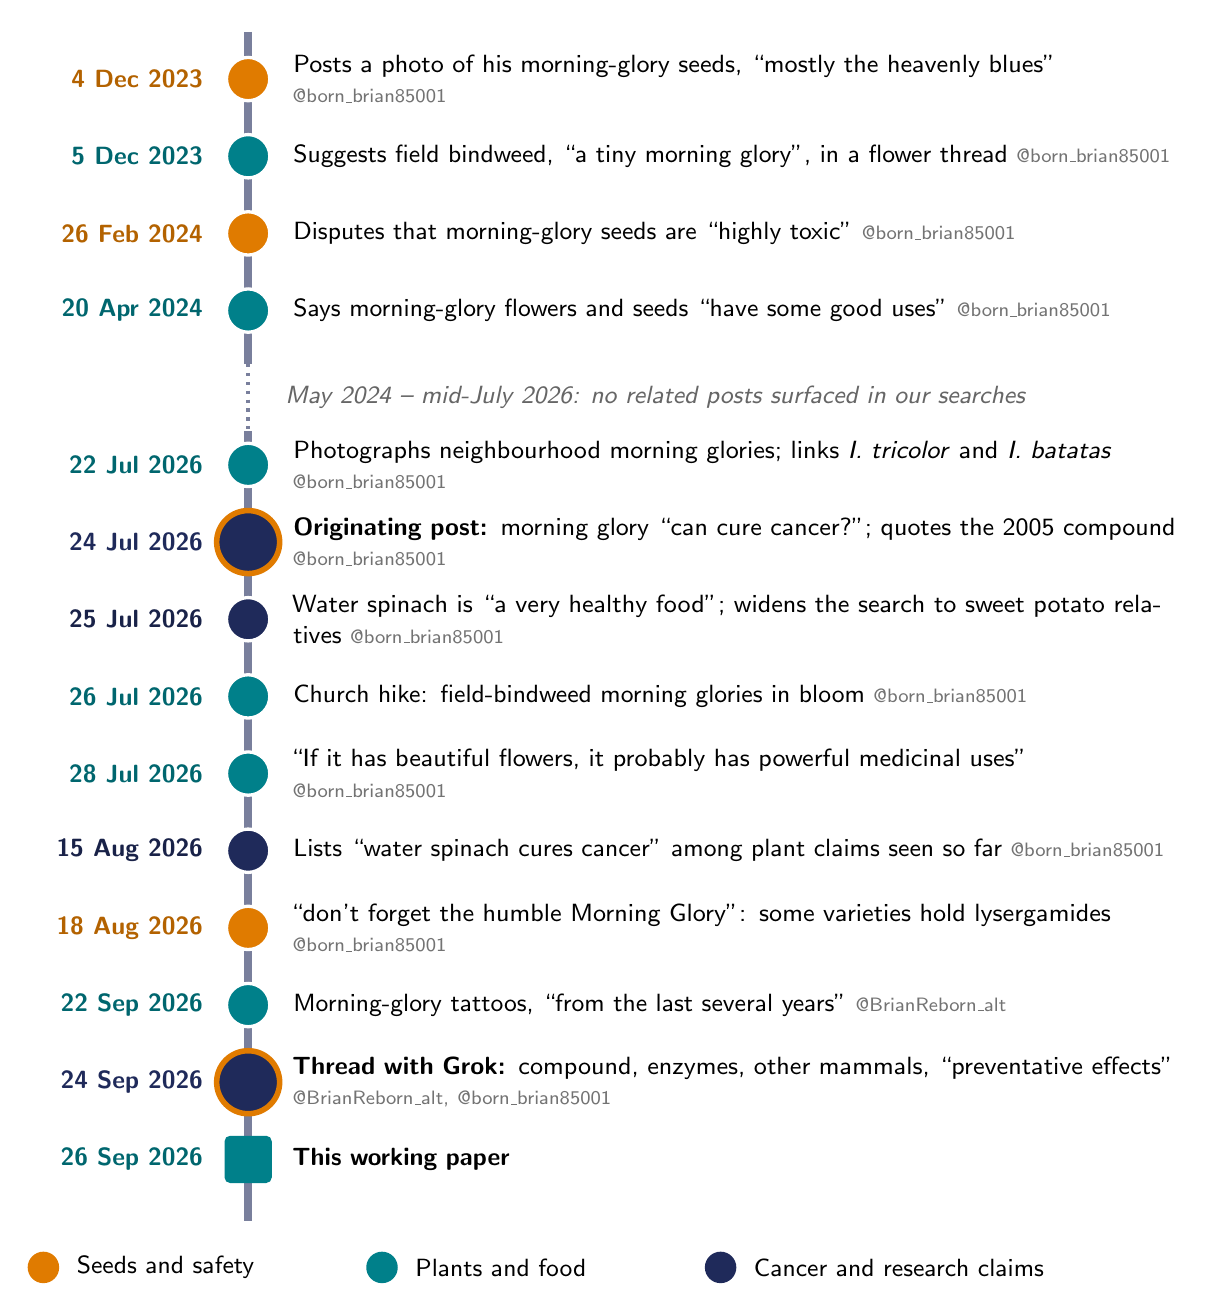
\begin{tikzpicture}[font=\sffamily, x=1cm, y=1cm]
% type colours: orange = seeds / safety-relevant, teal = plants & food, navy = cancer / research claim
\def\rowh{0.98}
\draw[navy!60, line width=3pt] (0,0.6) -- (0,-4*\rowh+0.3);
\draw[navy!60, line width=3pt] (0,-4*\rowh-0.55) -- (0,-15*\rowh+0.2);
% gap marker
\draw[navy!60, line width=1.2pt, dotted] (0,-4*\rowh+0.3) -- (0,-4*\rowh-0.55);
\node[font=\sffamily\itshape\small, text=black!60, anchor=west] at (0.35,-4*\rowh-0.12) {May 2024 -- mid-July 2026: no related posts surfaced in our searches};
\newcommand{\ev}[5]{% row, date, colour, short label, handle
  \node[circle, fill=#3, draw=white, line width=1.2pt, minimum size=5.5mm] at (0,-#1*\rowh) {};
  \node[anchor=east, font=\sffamily\bfseries\small, text=#3!80!black] at (-0.45,-#1*\rowh) {#2};
  \node[anchor=west, text width=11.2cm, font=\sffamily\small] at (0.45,-#1*\rowh) {#4 {\color{black!55}\scriptsize #5}};}
\ev{0}{4 Dec 2023}{orange}{Posts a photo of his morning-glory seeds, ``mostly the heavenly blues''}{@born\_brian85001}
\ev{1}{5 Dec 2023}{teal}{Suggests field bindweed, ``a tiny morning glory'', in a flower thread}{@born\_brian85001}
\ev{2}{26 Feb 2024}{orange}{Disputes that morning-glory seeds are ``highly toxic''}{@born\_brian85001}
\ev{3}{20 Apr 2024}{teal}{Says morning-glory flowers and seeds ``have some good uses''}{@born\_brian85001}
\ev{5}{22 Jul 2026}{teal}{Photographs neighbourhood morning glories; links \emph{I.~tricolor} and \emph{I.~batatas}}{@born\_brian85001}
\node[circle, fill=navy, draw=orange, line width=2pt, minimum size=8mm] at (0,-6*\rowh) {};
\node[anchor=east, font=\sffamily\bfseries\small, text=navy] at (-0.45,-6*\rowh) {24 Jul 2026};
\node[anchor=west, text width=11.2cm, font=\sffamily\small] at (0.45,-6*\rowh) {\textbf{Originating post:} morning glory ``can cure cancer?''; quotes the 2005 compound {\color{black!55}\scriptsize @born\_brian85001}};
\ev{7}{25 Jul 2026}{navy}{Water spinach is ``a very healthy food''; widens the search to sweet potato relatives}{@born\_brian85001}
\ev{8}{26 Jul 2026}{teal}{Church hike: field-bindweed morning glories in bloom}{@born\_brian85001}
\ev{9}{28 Jul 2026}{teal}{``If it has beautiful flowers, it probably has powerful medicinal uses''}{@born\_brian85001}
\ev{10}{15 Aug 2026}{navy}{Lists ``water spinach cures cancer'' among plant claims seen so far}{@born\_brian85001}
\ev{11}{18 Aug 2026}{orange}{``don't forget the humble Morning Glory'': some varieties hold lysergamides}{@born\_brian85001}
\ev{12}{22 Sep 2026}{teal}{Morning-glory tattoos, ``from the last several years''}{@BrianReborn\_alt}
\node[circle, fill=navy, draw=orange, line width=2pt, minimum size=8mm] at (0,-13*\rowh) {};
\node[anchor=east, font=\sffamily\bfseries\small, text=navy] at (-0.45,-13*\rowh) {24 Sep 2026};
\node[anchor=west, text width=11.2cm, font=\sffamily\small] at (0.45,-13*\rowh) {\textbf{Thread with Grok:} compound, enzymes, other mammals, ``preventative effects'' {\color{black!55}\scriptsize @BrianReborn\_alt, @born\_brian85001}};
\node[rectangle, rounded corners=2pt, fill=teal, minimum size=6mm] at (0,-14*\rowh) {};
\node[anchor=east, font=\sffamily\bfseries\small, text=teal!80!black] at (-0.45,-14*\rowh) {26 Sep 2026};
\node[anchor=west, text width=11.2cm, font=\sffamily\small] at (0.45,-14*\rowh) {\textbf{This working paper}};
% legend
\begin{scope}[shift={(-2.6,-15.4*\rowh)}]
\foreach \c/\t [count=\i] in {orange/Seeds and safety,teal/Plants and food,navy/Cancer and research claims}{
  \node[circle, fill=\c, minimum size=4mm] at (\i*4.3-4.3,0) {}; \node[anchor=west, font=\sffamily\small] at (\i*4.3-4.0,0) {\t};}
\end{scope}
\end{tikzpicture}
\end{adjustbox}
\caption{Body of work timeline: related public posts by the first author, dated in Pacific Time. Circle colour shows the theme; the two large circles are the originating post and the 24 September thread. Short labels are paraphrases, except words in quotation marks, which are verbatim. Full texts and links are in Table~\ref{tab:timeline} and \texttt{artifacts/brian-quotes.json}.}
\label{fig:timeline}
\end{figure}

{\small
\renewcommand{\arraystretch}{1.25}
\begin{longtable}{@{}>{\raggedright\arraybackslash}p{1.7cm} >{\raggedright\arraybackslash}p{9.3cm} >{\raggedright\arraybackslash}p{4.1cm}@{}}
\caption{The first author's related posts, verbatim (leading reply @-handles omitted). Dates are PT.}\label{tab:timeline}\\
\toprule
\textbf{Date} & \textbf{Post (exact text)} & \textbf{Account / link}\\
\midrule\endfirsthead
\toprule
\textbf{Date} & \textbf{Post (exact text)} & \textbf{Account / link}\\
\midrule\endhead
\bottomrule\endfoot
\TLrow{1731688059152834729}
\TLrow{1732071882491416995}
\TLrow{1762103456179892669}
\TLrow{1781568832605188543}
\TLrow{2079981200429780998}
\TLrow{2080792129669038191}
\TLrow{2080799123910037944}
\TLrow{2080812768035492294}
\TLrow{2080815533545627794}
\TLrow{2081172947277128130}
\TLrow{2082136462024454196}
\TLrow{2088459658923311197}
\TLrow{2089555749815075008}
\TLrow{2102607071535669594}
\TLrow{2103075947415269404}
\end{longtable}
}

\noindent Three of these posts bear on the paper's claims and get a direct response. On 26~February 2024 the author called the toxicity of morning-glory \emph{seeds} ``a lie,'' and on 18~August 2026 he wrote that some varieties ``have amazing healing properties that obviously pharma doesn't want you to know of.'' The literature does not support either claim. Seeds of the ornamental species contain d-lysergamide, and case reports describe serious adverse effects~\cite{juszczak2013}. We found no evidence of suppression, only an evidence base that is still at the cell-and-animal stage (Figure~\ref{fig:ladder}). The 15~August 2026 post is sceptical rather than promotional, and treats ``water spinach cures cancer'' as one claim in a series. That scepticism is the spirit in which this paper narrows the originating statement to a modest, testable hypothesis.

% =====================================================================
\section{Working Thesis}
\label{sec:thesis}

\begin{thesisbox}
\textbf{Working thesis (hypothesis, not a finding).}\quad
\emph{Regular dietary intake of water spinach (\emph{Ipomoea aquatica}) plausibly contributes a modest cancer-preventive effect via its flavonoid glycosides.}
\end{thesisbox}

\noindent The thesis answers the author's own question from the thread (``Do we agree that hypothetically we should have some expectation of cancer preventative effects?'') with a bounded yes:
\begin{itemize}[itemsep=2pt]
\item It is a \textbf{working hypothesis}. It is \textbf{not} a claim that any morning glory cures cancer, and it is not medical advice.
\item There is \textbf{no human study of water spinach and cancer}. The only human association we found that involves water spinach, as ``ong choy'' grouped with other leaves in an exploratory case-control study, points toward \emph{higher} risk of premalignant cervical lesions~\cite{hernandez2004} (Section~\ref{sec:counter}).
\item ``Modest'' is calibrated by the epidemiology of vegetables and flavonoids as a whole. There, the association with total cancer is small (a summary relative risk of 0.97 per 200~g/day of fruit and vegetables~\cite{aune2017}) and sometimes null~\cite{wang2009,takachi2008}.
\item The thesis concerns cooked \emph{leaves and stems of \Ia{}} grown in clean water. It does \textbf{not} extend to seeds of ornamental morning glories, to concentrated extracts, or to isolated resin glycosides.
\end{itemize}

% =====================================================================
\section{The Morning Glory Family at a Glance}
\label{sec:family}

Table~\ref{tab:family} replaces the Grok chart (whose moonflower image was wrong) with the six species it showed, plus the ornamental seed species that matter for safety. Only the first two rows are foods in ordinary use. The thesis concerns the first row only.

\begin{table}[H]
\centering\small
\caption{Morning glories re-tabulated with an edible-versus-toxic marker. Food status is common usage, not a safety endorsement. A grey marker means only that the species is not evaluated as food here.}
\label{tab:family}
\newcommand{\edible}{\tikz[baseline=-0.6ex]{\node[circle, fill=teal, text=white, inner sep=1.2pt, font=\sffamily\bfseries\small] {\ding{51}};}}
\newcommand{\toxic}{\tikz[baseline=-0.6ex]{\node[regular polygon, regular polygon sides=3, fill=red!75!black, text=white, inner sep=0.6pt, font=\sffamily\bfseries\scriptsize] {!};}}
\newcommand{\notfood}{\tikz[baseline=-0.6ex]{\node[circle, fill=black!35, text=white, inner sep=1.6pt, font=\sffamily\bfseries\small] {--};}}
\renewcommand{\arraystretch}{1.35}
\begin{tabularx}{\textwidth}{@{}c >{\raggedright\arraybackslash}p{2.6cm} >{\raggedright\arraybackslash}p{3.0cm} >{\raggedright\arraybackslash}X@{}}
\toprule
 & \textbf{Species} & \textbf{Common name} & \textbf{What people use it for, and its place in this paper}\\
\midrule
\rowcolor{teallight}\edible & \emph{I.~aquatica} & Water spinach, kangkung, ong choy & Leaves and stems eaten as an everyday green across Asia~\cite{thu2004}. \textbf{The subject of the thesis.} Buy from clean water and cook it (Section~\ref{sec:safety}).\\
\edible & \emph{I.~batatas} & Sweet potato & Roots and leaves (greens) eaten~\cite{karna2011,jin2007}. Same genus; supporting evidence only.\\
\notfood & \emph{I.~alba} & Moonflower & Ornamental vine. Not evaluated as food here.\\
\notfood & \emph{I.~quamoclit} & Cypress vine & Ornamental vine. Not evaluated as food here.\\
\notfood & \emph{I.~pes-caprae} & Beach morning glory & Coastal plant with traditional medicinal uses~\cite{meira2012}. Not evaluated as food here.\\
\notfood & \emph{I.~arborescens} & Tree morning glory & Ornamental tree or shrub. Not evaluated as food here.\\
\rowcolor{red!6}\toxic & \emph{I.~tricolor}, \emph{I.~violacea}, \emph{I.~purpurea} (seeds) & Garden morning glory, e.g.\ ``Heavenly Blue'' & Seeds contain d-lysergamide (LSA) and are taken as a drug, with serious adverse effects~\cite{juszczak2013}. \textbf{Toxic; not food.}\\
\bottomrule
\multicolumn{4}{@{}l}{\small \edible\ eaten as food \qquad \notfood\ not a food in this paper (no claim about safety) \qquad \toxic\ toxic, not food}\\
\end{tabularx}

\end{table}

% =====================================================================
\section{Chronological Literature Core}
\label{sec:literature}

Entries are strictly chronological, and each carries its reference number from the bibliography. Each gives a one-sentence summary and a causal-role sentence tying it to the thesis, to a stop-gap (SG1--SG3), to a mechanism step (M1--M10, Section~\ref{sec:mechanism}) or to the counter-evidence. Full details, DOIs and PMIDs are in the bibliography. The single arXiv item is a \textbf{preprint (not peer reviewed)}, used only for framing.

\subsection{Foundations and cautions (1977--2000)}
\begin{litlist}
\litentry{bjeldanes1977}{Bjeldanes \& Chang (1977)}{In Ames tests, quercetin was mutagenic (more so with metabolic activation), whereas dihydroquercetin (taxifolin), rutin and the other flavonoids tested were not.}{Distinguishes the water-spinach aglycone (taxifolin) from quercetin on genotoxicity, a point in its favour and a reason not to treat the two as interchangeable.}

\litentry{alphatocopherolbetac1994}{ATBC Cancer Prevention Study Group (1994)}{In 29{,}133 male smokers, $\beta$-carotene supplements increased lung-cancer incidence (by about 18\%) instead of lowering it.}{The central cautionary tale for SG3: an ``antioxidant from vegetables'' given as a supplement caused harm, so food-level hypotheses must not be turned into pills.}

\litentry{hollman1995}{Hollman et al. (1995)}{In nine ileostomy volunteers, 52\% of quercetin glucosides from onions were absorbed, against 24\% of pure quercetin aglycone and 17\% of rutinoside.}{Establishes that glucose conjugation \emph{enhances} human small-intestinal uptake, the first link from a glucoside-bearing vegetable to systemic exposure (E2).}

\litentry{omenn1996}{Omenn et al. (1996)}{In CARET, $\beta$-carotene plus vitamin~A raised lung-cancer incidence (RR 1.28) and mortality in high-risk adults.}{A second harmful antioxidant prevention trial, reinforcing that SG3 concerns whole foods, not isolated compounds.}

\litentry{woo1997}{Woo et al. (1997)}{In 728 Hong Kong Chinese adults, those who ate water spinach twice or more a week had higher mean plasma total antioxidant capacity.}{The only human biomarker datum for water spinach we found. It hints that eating it changes blood chemistry, but it is cross-sectional and unrelated to cancer.}

\litentry{day1998}{Day et al. (1998)}{Cell-free extracts of human small intestine and liver rapidly deglycosylated quercetin 4$'$-glucoside and several flavonoid 7-glucosides, but left quercetin 3-glucoside, 3,4$'$-diglucoside and rutinosides unchanged.}{Shows that human CBG cuts 7-\emph{O}-glucosides (M2), and that it has substrate limits, including at the 3-position, which bear directly on the diglucoside.}

\litentry{kasturi1998}{Kasturi et al. (1998)}{In a phase~I trial of intravenous 4-ipomeanol in 44 lung-cancer patients, the dose-limiting toxicity was hepatic and there were no objective responses.}{A cautionary node for SG3: a toxin named for \emph{Ipomoea} that looked promising pre-clinically failed in humans; cytotoxicity is not cure.}

\litentry{day2000}{Day et al. (2000)}{Lactase-phlorizin hydrolase purified from sheep small intestine hydrolysed quercetin-4$'$-glucoside, quercetin-3-glucoside and isoflavone glucosides.}{Supplies the luminal enzyme for M2 and, because it is a sheep enzyme, grounds the mammalian homology used in SG2.}
\end{litlist}

\subsection{Absorption, chemistry and first human signals (2001--2008)}
\begin{litlist}
\litentry{braune2001}{Braune et al. (2001)}{The human gut anaerobe \emph{Eubacterium ramulus} degraded quercetin via taxifolin to 3,4-dihydroxyphenylacetic acid, and converted added taxifolin the same way.}{Gut bacteria can both free and destroy taxifolin (M3). The bacterial route around the $\alpha$-link may therefore deliver phenolic acids rather than taxifolin.}

\litentry{graczyk2001}{Graczyk et al. (2001)}{The giant intestinal fluke \emph{Fasciolopsis buski} is transmitted by eating raw aquatic plants grown in contaminated ponds.}{A safety limit: raw water greens carry parasite risk, so any dietary recommendation must specify cooking.}

\litentry{gothberg2002}{G\"othberg et al. (2002)}{Water spinach grown around Bangkok accumulated mercury, cadmium and lead, especially near polluted water.}{A safety limit: contaminant load depends on the growing water and could offset any benefit.}

\litentry{knekt2002}{Knekt et al. (2002)}{In 10{,}054 Finnish adults, men with higher quercetin intake had lower lung-cancer incidence (RR 0.42, highest vs lowest quartile).}{An early human node (E4) linking dietary flavonols to lower cancer risk; associational.}

\litentry{berrin2003}{Berrin et al. (2003)}{A homology model and mutagenesis of human CBG showed that its activity on flavonoid glucosides depends on the aglycone, the sugar and the linkage, and identified aglycone-binding residues.}{Gives the structural basis for testing whether CBG accepts the diglucoside (M2), an open gap.}

\litentry{day2003}{Day et al. (2003)}{In rat everted jejunum, quercetin-3-glucoside was absorbed only after LPH hydrolysis.}{Shows the rodent gut uses the same enzyme route as human tissue, so rodent feeding data can bear on humans (SG2).}

\litentry{malalavidhane2003}{Malalavidhane et al. (2003)}{Shredded \Ia{} leaves lowered fasting glucose in diabetic rats, and a single blended dose lowered 2-h glucose in type~2 diabetic patients.}{Shows that the eaten plant has measurable biological effects in rats and people. The effect is not related to cancer, but it makes a feeding study feasible.}

\litentry{nemeth2003}{N\'emeth et al. (2003)}{LPH and CBG were isolated from human small-intestinal mucosa and hydrolysed flavonoid glycosides, with large inter-individual variation.}{Confirms both enzymes in human tissue (M2); the variation implies any benefit would differ between people.}

\litentry{hernandez2004}{Hernandez et al. (2004)}{In an exploratory Honolulu case-control study (122 cases, 183 controls), a lignan-source food group listed as ``taro leaves/ong choy/marunggay'' was \emph{positively} associated with premalignant cervical lesions.}{The only human cancer-related association involving water spinach that we found, and it points the wrong way. It is weak and grouped, but it is disclosed as counter-evidence.}

\litentry{kroon2004}{Kroon et al. (2004)}{Argued that \emph{in vitro} polyphenol studies should test the conjugates found in blood, at concentrations of about 0.1--10~$\mu$mol/L reached after a polyphenol-rich meal.}{The methodological core of SG1: most cell studies cited here used aglycones at far higher concentrations.}

\litentry{thu2004}{Thu et al. (2004)}{Water spinach supplied about 45\% of a mean polyphenol intake of 595~mg catechin equivalents per day in northern Vietnam.}{Anchors dose realism for SG1: high consumers take in hundreds of milligrams of polyphenols a day, much of it from this plant.}

\litentry{manach2005}{Manach et al. (2005)}{Across 97 human bioavailability studies, total plasma polyphenol metabolites ranged from 0 to 4~$\mu$mol/L after about 50~mg aglycone equivalents.}{The quantitative anchor for SG1 and M5: realistic plasma levels are low-micromolar at most and consist of conjugates.}

\litentry{prasad2005}{Prasad et al. (2005)}{Activity-guided fractionation of \Ia{} leaves yielded an antioxidant (DPPH EC$_{50}$ 83~$\mu$g/mL) tentatively identified as \DQG.}{The isolation paper for the key compound (M1). Its $\alpha$-linkage at C-3 is the basis of the $\alpha$-link caveat (M3).}

\litentry{prasad2005b}{Prasad et al. (2005b)}{The purified diglucoside, a crude leaf extract and a fraction were tested on Vero (normal), HEp-2 and A-549 cells. The pure compound's CTC$_{50}$ values were 387, 156 and 394 (reported as mg/mL), and the crude extract was more potent.}{This is the ``2005 weak \emph{in vitro}'' study of the thread. The compound is weakly and non-selectively cytotoxic, so direct cell killing by the parent glycoside is not a plausible dietary mechanism.}

\litentry{cao2007}{Cao et al. (2007)}{Ipomoeassin F, a resin glycoside from \emph{I.~squamosa} leaves, inhibited A2780 ovarian cancer cells with an IC$_{50}$ of 0.036~$\mu$M.}{The genus makes potent cytotoxins; these are pharmacological, not dietary, and lie outside the chain.}

\litentry{jin2007}{Jin et al. (2007)}{In a Taiwanese case-control study (301 cases, 1{,}204 controls), the highest tertile of sweet-potato-leaf intake was associated with lower lung-cancer risk (adjusted OR 0.43--0.65).}{The closest human cancer datum for an edible \emph{Ipomoea} leaf. It concerns a sister species and is case-control, but it points the thesis's way (E4).}

\litentry{kottra2007}{Kottra \& Daniel (2007)}{Flavonoid glycosides were not transported by the human sodium-glucose transporter SGLT1 expressed in oocytes.}{Removes the intact-uptake route, leaving deglycosylation (M2, M3) as the main path to absorption.}

\litentry{lee2007}{Lee et al. (2007)}{Taxifolin induced quinone reductase in HCT116 colon cells with low cytotoxicity and, at 60~$\mu$M, activated antioxidant-response-element genes such as \emph{NQO1} and \emph{GSTM1}.}{The mechanistic node for M7: taxifolin behaves as a phase-II-inducing chemopreventive, which fits prevention better than cytotoxicity.}

\litentry{neufert2007}{Neufert et al. (2007)}{A protocol for azoxymethane (AOM) colon carcinogenesis in mice, alone (tumours within about 30 weeks) or with dextran sodium sulfate (DSS; multiple tumours within about 10 weeks), with tumour scoring systems.}{The methods basis of the proposed animal feeding study (Section~\ref{sec:animal}).}

\litentry{vuong2007}{Vuong et al. (2007)}{Water spinach grown in Phnom Penh wastewater lakes was heavily contaminated with faecal bacteria and protozoan parasites.}{A safety limit on wastewater-grown produce.}

\litentry{bobe2008}{Bobe et al. (2008)}{In the Polyp Prevention Trial cohort, high flavonol intake was associated with lower recurrence of advanced colorectal adenoma (OR 0.24).}{A human signal for flavonols and a pre-cancerous endpoint (E4), from a secondary analysis.}

\litentry{egert2008}{Egert et al. (2008)}{Quercetin at 50--150~mg/day for two weeks raised plasma quercetin dose-dependently (median peak 431~nmol/L at 150~mg) without changing oxidative or inflammatory markers.}{Even supplement-level flavonol intake gives sub-micromolar plasma levels (SG1).}

\litentry{luo2008}{Luo et al. (2008)}{Of 12 compounds tested on OVCAR-3 cells, taxifolin, quercetin and others inhibited growth, but taxifolin was the weakest VEGF inhibitor, attributed to its missing C2=C3 double bond.}{Grok-cited and verified. Dihydroquercetin is active but not equivalent to quercetin.}

\litentry{marcussen2008}{Marcussen et al. (2008)}{Element contents of wastewater-grown water spinach in Hanoi were mostly below food-safety limits.}{A partly reassuring counterpoint: contamination is site-specific, not inherent.}

\litentry{takachi2008}{Takachi et al. (2008)}{In 77{,}891 Japanese adults, vegetable intake was not associated with total cancer (HR 0.94, 95\% CI 0.84--1.05).}{Null Asian cohort evidence for vegetables and total cancer, tempering E4.}
\end{litlist}

\subsection{Mechanisms, models and mixed epidemiology (2009--2016)}
\begin{litlist}
\litentry{wang2009}{Wang et al. (2009)}{In 38{,}408 women, intake of flavonols and flavones was not associated with total or site-specific cancer.}{A large null cohort for flavonols (counter-evidence to E4).}

\litentry{murota2010}{Murota et al. (2010)}{Adding $\alpha$-linked glucose units to the sugar of quercetin 3-glucoside increased its bioavailability in humans.}{Human evidence that $\alpha$-glucosyl sugars on a flavonoid glucoside do not block absorption, which softens, but does not settle, the $\alpha$-link caveat (M3).}

\litentry{karna2011}{Karna et al. (2011)}{A polyphenol-rich sweet-potato greens extract inhibited prostate-cancer cells and, orally at 400~mg/kg, reduced PC-3 xenograft growth by about 69\% in mice.}{An oral anticancer effect of an \emph{Ipomoea} leaf extract, at a dose far above diet (SG1) and in a treatment model (SG3).}

\litentry{klein2011}{Klein et al. (2011)}{In SELECT, vitamin~E supplements increased prostate-cancer risk (HR 1.17).}{Another antioxidant-supplement harm, bounding SG3.}

\litentry{bjelakovic2012}{Bjelakovic et al. (2012)}{A Cochrane review found that antioxidant supplements do not reduce mortality, and some increase it.}{High-level cautionary evidence against extrapolating from ``antioxidant'' to benefit (M9).}

\litentry{jin2012}{Jin et al. (2012)}{A Cochrane review found insufficient and conflicting evidence that dietary flavonoids prevent colorectal neoplasms.}{A high-level inconclusive verdict limiting E4.}

\litentry{meira2012}{Meira et al. (2012)}{A review of the genus \emph{Ipomoea}: traditional uses, chemistry and biology, including the 2005 water-spinach cytotoxicity data.}{The review the first author quoted on 24~July 2026. It reports the C-3 sugar as $\beta$ and the CTC$_{50}$ values in mg/mL.}

\litentry{oi2012}{Oi et al. (2012)}{Taxifolin bound and inhibited EGFR and PI3K and, applied topically, suppressed UV-induced skin tumours in mice.}{The model evidence for M6, by a topical rather than dietary route (SG1, SG2).}

\litentry{zheng2012}{Zheng et al. (2012)}{Quercetin inhibited A549 cells (IC$_{50}$ about 1.0--1.4~$\mu$mol/L) and, at 8~mg/kg, A549 xenografts in mice.}{Grok-cited and verified; one of the few potencies near the diet-achievable range.}

\litentry{deng2013}{Deng et al. (2013)}{Quercetin inhibited MCF-7 proliferation, induced G0/G1 arrest and apoptosis, and reduced survivin.}{Grok-cited and verified; a representative \emph{in vitro} node.}

\litentry{juszczak2013}{Juszczak \& Swiergiel (2013)}{User and case reports on recreational ingestion of \emph{I.~tricolor}, \emph{I.~violacea}, \emph{I.~purpurea} and \emph{Argyreia nervosa} seeds for d-lysergamide describe adverse effects, including suicidal ideation.}{Sets the safety boundary: ornamental seeds are drugs and toxins, outside the thesis.}

\litentry{akhmetzhanov2014}{Akhmetzhanov \& Hochberg (2014) \prelim}{A stochastic and mean-field model predicts that constant, low-impact chemoprevention can control small neoplasms while limiting resistance.}{Framing for SG3: a small, persistent effect is the relevant quantity for prevention.}

\litentry{fan2014}{Fan et al. (2014)}{Eleven new resin glycosides (aquaterins) from whole \Ia{} plants; the most active inhibited HepG2 cells (IC$_{50}$ 2.4~$\mu$M).}{The edible species carries cytotoxic resin glycosides, a second compound class whose dietary exposure is unknown.}

\litentry{cincin2015}{Cincin et al. (2015)}{Quercitrin caused apoptosis in DLD-1 colon cancer cells.}{Grok-cited and verified; rhamnosides need bacterial deglycosylation \emph{in vivo}.}

\litentry{manigandan2015}{Manigandan et al. (2015)}{In DMH-induced mouse colon carcinogenesis, taxifolin raised Nrf2 and lowered NF-$\kappa$B, TNF-$\alpha$, COX-2, $\beta$-catenin and cyclin~D1.}{The model evidence for M7 and M8, systemic and colon-specific (SG2).}

\litentry{lawal2016}{Lawal et al. (2016)}{LC-MS/MS of three \Ia{} cultivars tentatively identified quercetin glycosides (including a 3,7-diglucoside) and caffeoylquinic acids; the dihydroquercetin diglucoside was not reported.}{Challenges M1: the dominant flavonoids may be quercetin glycosides, and content varies by cultivar.}

\litentry{yang2016}{Yang et al. (2016)}{In rats, the oral absolute bioavailability of taxifolin was 0.49\% (0.75\% as a nanodispersion).}{A key SG1 limit on M4: little free taxifolin reaches blood after oral dosing.}
\end{litlist}

\subsection{Quantification, epidemiology, safety and the plant itself (2017--2026)}
\begin{litlist}
\litentry{aune2017}{Aune et al. (2017)}{A dose-response meta-analysis of prospective studies found a summary RR of 0.97 for total cancer per 200~g/day of fruit and vegetables.}{Sets the epidemiological ceiling for ``modest'' (E4).}

\litentry{grosso2017}{Grosso et al. (2017)}{A meta-analysis of observational studies found prospective evidence for flavonoid intake and cancer largely inconclusive, apart from isoflavones.}{Marks how weak flavonoid-specific epidemiology still is.}

\litentry{hashemzaei2017}{Hashemzaei et al. (2017)}{Quercetin at 10--120~$\mu$M induced apoptosis in nine tumour cell lines and reduced tumour volume in mice.}{Grok-cited and verified; its concentrations illustrate the SG1 gap.}

\litentry{hefnygad2018}{Hefny Gad et al. (2018)}{Chromatographic fingerprinting of \Ia{} identified flavonol glycosides including rutin and nicotiflorin.}{Confirms flavonol glycosides in the plant (M1), including rutinosides that need bacterial deglycosylation.}

\litentry{bondonno2019}{Bondonno et al. (2019)}{In 56{,}048 Danish adults followed for 23 years, moderate habitual flavonoid intake was associated with lower all-cause and cancer mortality, plateauing near 500~mg/day.}{The strongest human node for E4; associational.}

\litentry{sunil2019}{Sunil \& Xu (2019)}{A review of taxifolin finds anticancer activity prominent in models and calls for pharmacokinetic and randomised clinical studies.}{States plainly that clinical data for the aglycone are missing.}

\litentry{hisaka2020}{Hisaka et al. (2020)}{Quercetin (0--100~$\mu$M) suppressed proliferation of 13 liver cancer cell lines.}{Grok-cited and verified; broadens the \emph{in vitro} base.}

\litentry{perciedusert2020}{Percie du Sert et al. (2020)}{The ARRIVE 2.0 guidelines for reporting animal research, with an ``Essential 10'' minimum set.}{The reporting standard for the proposed animal feeding study.}

\litentry{shi2020}{Shi et al. (2020)}{In rats, the oral absolute bioavailability of astilbin (a taxifolin 3-\emph{O}-glycoside) was about 1.2\%.}{The closest pharmacokinetic analogue of a taxifolin 3-glycoside: intact exposure is about 1\% (M4).}

\litentry{wang2020}{Wang et al. (2020)}{Taxifolin at 25--100~$\mu$M suppressed stemness and EMT in lung cancer cells and inhibited A549 xenografts.}{Grok-cited and verified; taxifolin-specific, at concentrations that mark the SG1 gap.}

\litentry{hsieh2021}{Hsieh et al. (2021)}{In a Taiwanese national survey (2{,}592 adults), sweet-potato leaves/water spinach was one of the main flavonoid sources, and higher total flavonoid intake was associated with lower CRP (OR 0.61).}{Shows that water spinach is a measurable flavonoid source in a national survey and links flavonoid intake to an inflammation marker. A model for the proposed cross-sectional study.}

\litentry{papadimitriou2021}{Papadimitriou et al. (2021)}{An umbrella review found that few single food-cancer associations are supported by strong evidence.}{Tempers claims for any single vegetable.}

\litentry{thang2021}{Thang et al. (2021)}{Nitrate and heavy-metal hazard quotients from vegetables, including water spinach, and bivalves in Ho Chi Minh City exceeded 1 for some groups.}{Nitrate is itself a cancer-relevant exposure in leafy greens (safety limit).}

\litentry{sasikala2022}{Sasikala et al. (2022)}{Merromoside, a resin glycoside from \Ia{}, inhibited MCF-7 cells with an IC$_{50}$ of 182.8~$\mu$g/mL.}{Plant-derived activity only at very high concentrations (SG1).}

\litentry{toy2022}{Toy et al. (2022)}{\Ia{} resin-glycoside extracts inhibited pancreatic lipase \emph{in vitro} and were unstable at 90\,$^\circ$C.}{Cooking may destroy the resin glycosides, relevant to whether cytotoxic aquaterins survive in food.}

\litentry{saikia2023}{Saikia et al. (2023)}{UPLC-qTOF-MS/MS profiling of \Ia{} identified more than 65 compounds, mostly polyphenol glycosides, and the extracts prevented induced DNA damage \emph{in vitro}.}{Genoprotection (M9), the plant-level mechanism closest to prevention.}

\litentry{ramos2024}{Ramos et al. (2024)}{Quercetin and chrysin each reduced breast-cancer cell viability, and the combination enhanced cytotoxicity.}{Grok-cited and verified; flavonoid mixtures, as in foods, may act together.}

\litentry{wei2024}{Wei et al. (2024)}{Mendelian randomisation found no robust causal association between fruit or vegetable intake and gastrointestinal cancers.}{Causal-inference counter-evidence to E4.}

\litentry{parmenter2025}{Parmenter et al. (2025)}{In 124{,}805 UK Biobank participants, greater diversity of flavonoid intake was associated with lower risk of mortality and several chronic diseases, including cancer.}{Supports water spinach as one contributor to a diverse flavonoid diet (SG3).}

\litentry{huang2026}{Huang et al. (2026)}{Of 12 vegetables screened, sweet-potato leaves, water spinach and coriander were top candidates for inhibiting heterocyclic amine formation in charcoal-grilled pork; inhibition was 43--93\%, depending on the marinade.}{A non-systemic ``in the pan'' prevention route that bypasses SG1 entirely (Section~\ref{sec:mechanism}).}

\litentry{wu2026}{Wu et al. (2026)}{In Guangzhou leafy vegetables, the bioaccessibility-adjusted screening carcinogenic risk (mostly inorganic arsenic) for adults eating water spinach was $4.1\times10^{-3}$ raw and $2.2\times10^{-3}$ after boiling.}{The strongest safety limit: in contaminated regions the arsenic risk exceeds the usual $10^{-4}$ benchmark and could outweigh any flavonoid benefit.}
\end{litlist}

% =====================================================================
\section{Verification of Grok-Cited Studies and the 2005 Figures}
\label{sec:verification}

The first author asked Grok for the studies:

\BQ{2103096988892053875}

\noindent Each PMID Grok gave on 24 September was fetched from PubMed E-utilities (26 September 2026). Its title, abstract and cell lines were compared with Grok's one-line description, and its DOI was resolved at \url{https://doi.org/}. Table~\ref{tab:pmid} lists the results. The three identifiers singled out for checking (22200874, 24223637, 39146763) all check out. Items Grok gave without a PMID were not verified and are not cited. As Grok itself noted, these are \emph{in vitro} studies, not cross-sectional ones.

\begin{table}[H]
\centering\small
\caption{Verification of the twelve \emph{in vitro} studies Grok listed.}
\label{tab:pmid}
\begin{tabularx}{\textwidth}{@{}c l X l@{}}
\toprule
\# & \textbf{PMID} & \textbf{Grok's description $\rightarrow$ PubMed record} & \textbf{Status}\\
\midrule
1 & 22200874 & A549 lung $\rightarrow$ Zheng et al.\ 2012, quercetin in A-549~\cite{zheng2012} & Verified\\
2 & 24223637 & MCF-7 breast $\rightarrow$ Deng et al.\ 2013, quercetin/survivin in MCF-7~\cite{deng2013} & Verified\\
3 & 39146763 & Quercetin+chrysin, MDA-MB-231/MCF-7 $\rightarrow$ Ramos et al.\ 2024~\cite{ramos2024} & Verified\\
4 & --- & Quercetin on prostate LNCaP/DU-145/PC-3 (no PMID) & Not verified\\
5 & 19005980 & OVCAR-3 $\rightarrow$ Luo et al.\ 2008, 12 flavonoids incl.\ quercetin and taxifolin~\cite{luo2008} & Verified\\
6 & 25096395 & Quercitrin, DLD-1 $\rightarrow$ Cincin et al.\ 2015~\cite{cincin2015} & Verified\\
7 & 28677813 & CT-26/MCF-7 et al.\ $\rightarrow$ Hashemzaei et al.\ 2017, 9 lines~\cite{hashemzaei2017} & Verified\\
8 & 32566617 & Taxifolin, A549/H1975 $\rightarrow$ Wang et al.\ 2020~\cite{wang2020} & Verified\\
9 & --- & DHQ on SK-OV-3 ovarian (no PMID) & Not verified\\
10 & --- & Taxifolin on MDA-MB-231/4T1 (no PMID) & Not verified\\
11 & --- & Taxifolin on AGS gastric (no PMID) & Not verified\\
12 & 32727794 & 13 liver lines $\rightarrow$ Hisaka et al.\ 2020~\cite{hisaka2020} & Verified\\
\bottomrule
\end{tabularx}
\end{table}

\noindent \textbf{The 2005 figures, traced.} The review the first author quoted~\cite{meira2012} reports that the purified diglucoside gave CTC$_{50}$ values of 387 (normal Vero cells), 156 (HEp-2) and 394 (A-549) ``mg/mL,'' and that the crude extract and its column fraction gave 41--332, 46--114 and 44--230~mg/mL in the same cells, citing the 2005 short communication~\cite{prasad2005b}. Grok's ``40--400~mg/ml'' is a fair summary of these ranges. The unit is almost certainly a transcription of $\mu$g/mL: 387~mg/mL would be a solution that is nearly 40\% compound by weight. On the $\mu$g/mL reading (molar mass about 628~g/mol), the pure compound acted at roughly 250--630~$\mu$M, and it hit the normal cell line as hard as the cancer lines. Two further checks: the isolation paper exists~\cite{prasad2005}, and it reports the 3-\emph{O}-glucose as $\alpha$-linked and the structure as tentative, whereas the review, and therefore the author's quote, has $\beta$.

% =====================================================================
\section{Causal Chain with Labeled Stop-Gaps}
\label{sec:chain}

The chain has four empirical nodes (E1--E4) and three stop-gap bridges (SG1--SG3), and ends at the working thesis. Figure~\ref{fig:chain} draws it with icons and the paper's evidence colours. Figures~\ref{fig:pathway}--\ref{fig:ladder} then show the same argument four other ways: the journey from plate to cell, the molecule itself, the dose gap, and the ladder of evidence. The stop-gaps are \emph{reasoned bridges} that close empirical gaps. They are not experimental facts, and they are not treated as fatal obstacles; Section~\ref{sec:falsify} states what would make them fail.

\begin{figure}[tbp]
\centering
\begin{adjustbox}{max width=\linewidth}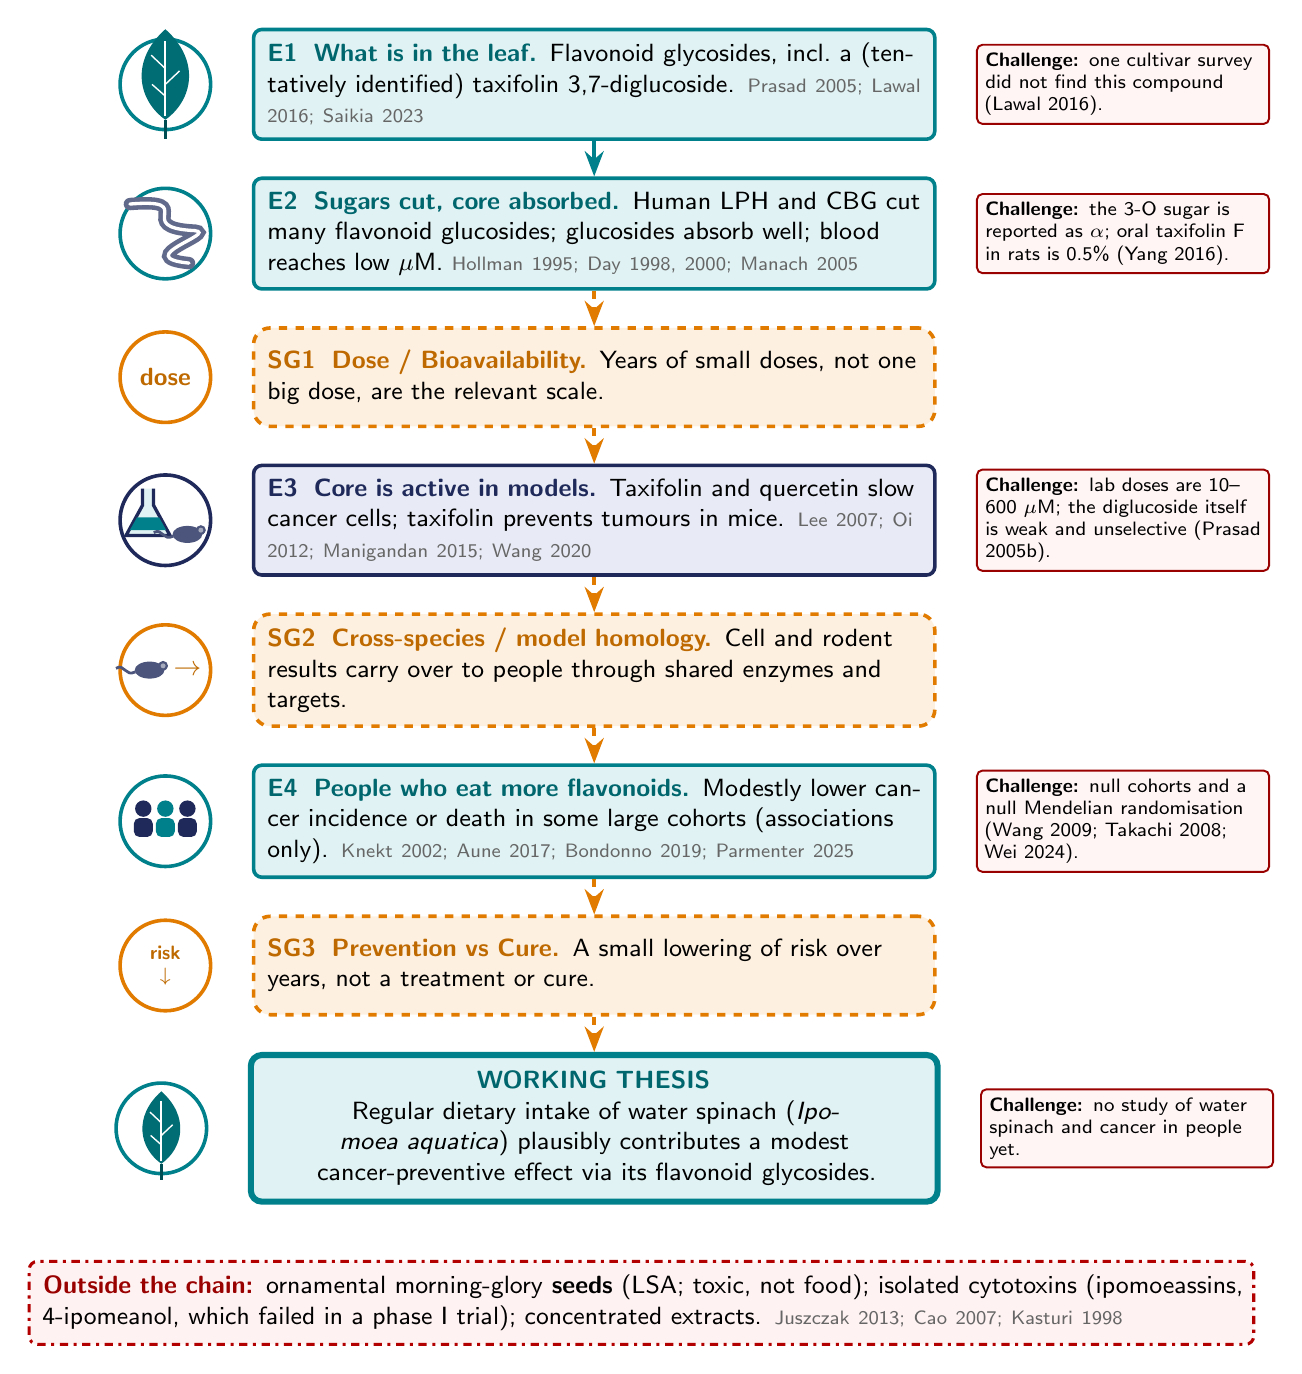
\begin{tikzpicture}[font=\sffamily\small, node distance=4.5mm,
  nd/.style={text width=8.3cm, align=left, inner sep=5pt, minimum height=1.25cm},
  ch/.style={draw=red!60!black, line width=0.7pt, fill=red!4, rounded corners=2pt, text width=3.5cm, align=left, font=\sffamily\scriptsize, inner sep=3pt},
  ic/.style={circle, draw=#1, line width=1.3pt, fill=white, minimum size=1.15cm}]
\node[nd, est] (e1) {\textbf{\color{teal!80!black}E1 \;What is in the leaf.} Flavonoid glycosides, incl.\ a (tentatively identified) taxifolin 3,7-diglucoside. {\scriptsize\color{black!60}Prasad 2005; Lawal 2016; Saikia 2023}};
\node[nd, est, below=of e1] (e2) {\textbf{\color{teal!80!black}E2 \;Sugars cut, core absorbed.} Human LPH and CBG cut many flavonoid glucosides; glucosides absorb well; blood reaches low $\mu$M. {\scriptsize\color{black!60}Hollman 1995; Day 1998, 2000; Manach 2005}};
\node[nd, prop, below=of e2] (sg1) {\textbf{\color{orange!85!black}SG1 \;Dose / Bioavailability.} Years of small doses, not one big dose, are the relevant scale.};
\node[nd, mod, below=of sg1] (e3) {\textbf{\color{navy}E3 \;Core is active in models.} Taxifolin and quercetin slow cancer cells; taxifolin prevents tumours in mice. {\scriptsize\color{black!60}Lee 2007; Oi 2012; Manigandan 2015; Wang 2020}};
\node[nd, prop, below=of e3] (sg2) {\textbf{\color{orange!85!black}SG2 \;Cross-species / model homology.} Cell and rodent results carry over to people through shared enzymes and targets.};
\node[nd, est, below=of sg2] (e4) {\textbf{\color{teal!80!black}E4 \;People who eat more flavonoids.} Modestly lower cancer incidence or death in some large cohorts (associations only). {\scriptsize\color{black!60}Knekt 2002; Aune 2017; Bondonno 2019; Parmenter 2025}};
\node[nd, prop, below=of e4] (sg3) {\textbf{\color{orange!85!black}SG3 \;Prevention vs Cure.} A small lowering of risk over years, not a treatment or cure.};
\node[text width=8.3cm, align=center, inner sep=6pt, draw=teal, line width=2.2pt, fill=teallight, rounded corners=4pt, below=of sg3] (th) {\textbf{\color{teal!80!black}WORKING THESIS}\\ Regular dietary intake of water spinach (\emph{Ipomoea aquatica}) plausibly contributes a modest cancer-preventive effect via its flavonoid glycosides.};
\foreach \a/\b/\s in {e1/e2/aest,e2/sg1/aprop,sg1/e3/aprop,e3/sg2/aprop,sg2/e4/aprop,e4/sg3/aprop,sg3/th/aprop}{\draw[\s] (\a) -- (\b);}
% icons
\node[ic=teal, left=5mm of e1] (i1) {}; \pic at ($(i1)+(0,-0.45)$) {leaf};
\node[ic=teal, left=5mm of e2] (i2) {}; \pic[scale=0.75] at (i2) {gut};
\node[ic=orange, left=5mm of sg1] (i3) {}; \node[font=\sffamily\bfseries\small, text=orange!85!black] at (i3) {dose};
\node[ic=navy, left=5mm of e3] (i4) {}; \pic[scale=0.7] at ($(i4)+(-0.22,0.05)$) {flask}; \pic[scale=0.45] at ($(i4)+(0.28,-0.18)$) {mouse};
\node[ic=orange, left=5mm of sg2] (i5) {}; \pic[scale=0.45] at ($(i5)+(-0.2,0)$) {mouse}; \node[font=\sffamily\bfseries, text=orange!85!black] at ($(i5)+(0.28,0)$) {$\rightarrow$};
\node[ic=teal, left=5mm of e4] (i6) {}; \pic[scale=0.8] at ($(i6)+(0,-0.2)$) {people};
\node[ic=orange, left=5mm of sg3] (i7) {}; \node[font=\sffamily\bfseries\scriptsize, text=orange!85!black, align=center] at (i7) {risk\\$\downarrow$};
\node[ic=teal, left=5mm of th] (i8) {}; \pic[scale=0.8] at ($(i8)+(0,-0.45)$) {leaf};
% challenges
\node[ch, right=5mm of e1] {\textbf{Challenge:} one cultivar survey did not find this compound (Lawal 2016).};
\node[ch, right=5mm of e2] {\textbf{Challenge:} the 3-O sugar is reported as $\alpha$; oral taxifolin F in rats is 0.5\% (Yang 2016).};
\node[ch, right=5mm of e3] {\textbf{Challenge:} lab doses are 10--600 $\mu$M; the diglucoside itself is weak and unselective (Prasad 2005b).};
\node[ch, right=5mm of e4] {\textbf{Challenge:} null cohorts and a null Mendelian randomisation (Wang 2009; Takachi 2008; Wei 2024).};
\node[ch, right=5mm of th] {\textbf{Challenge:} no study of water spinach and cancer in people yet.};
% exclusion
\node[tox, text width=15.2cm, align=left, inner sep=5pt, font=\sffamily\small, below=7mm of th.south, anchor=north, xshift=0.6cm] (ex) {\textbf{\color{red!60!black}Outside the chain:} ornamental morning-glory \textbf{seeds} (LSA; toxic, not food); isolated cytotoxins (ipomoeassins, 4-ipomeanol, which failed in a phase~I trial); concentrated extracts. {\scriptsize\color{black!60}Juszczak 2013; Cao 2007; Kasturi 1998}};
\end{tikzpicture}
\end{adjustbox}\\[4pt]
\evlegend
\caption{The causal chain from water-spinach chemistry to the working thesis. Teal boxes are established nodes (human data or human-tissue biochemistry); the navy box is supported by cell and animal models; dashed orange boxes are the three labelled stop-gap bridges. Red side notes give the strongest challenge to each node; the red dash-dot box lists what the chain explicitly excludes.}
\label{fig:chain}
\end{figure}

\begin{figure}[tbp]
\centering
\begin{adjustbox}{max width=\linewidth}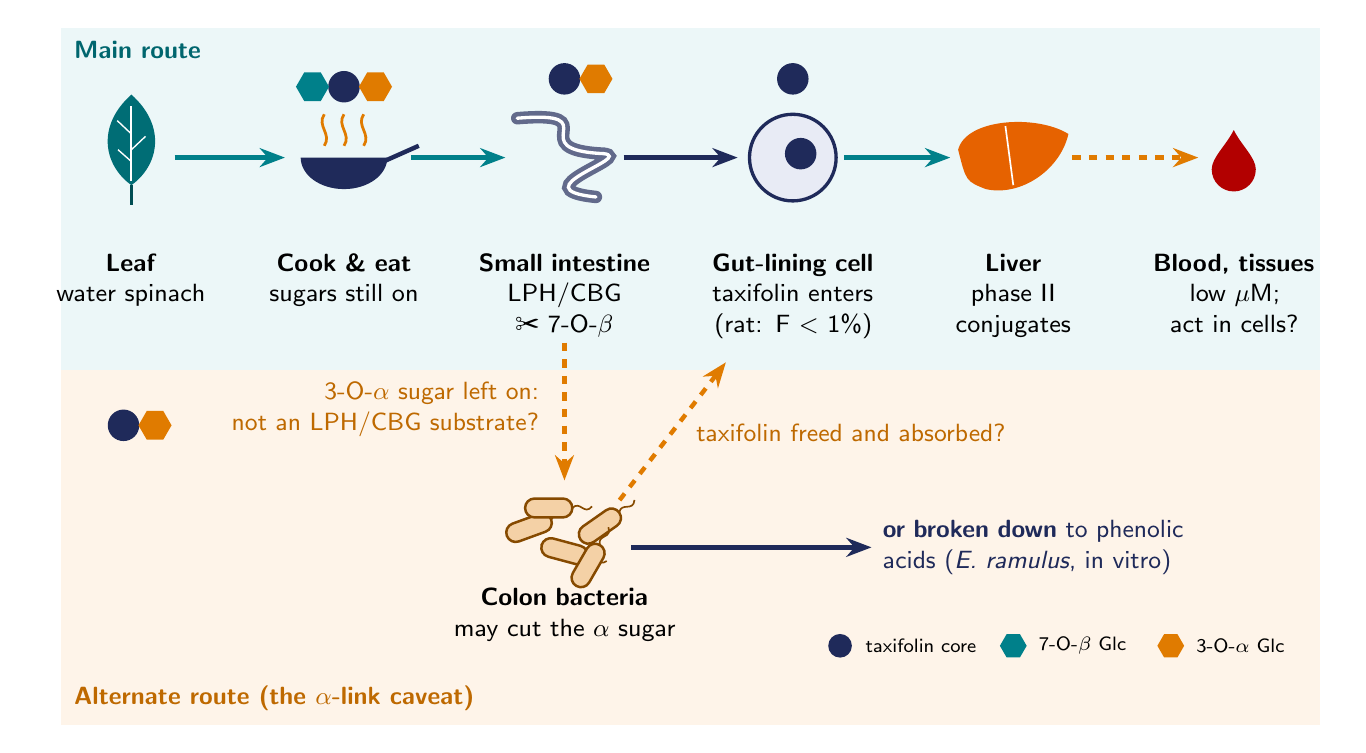
\begin{tikzpicture}[font=\sffamily, x=1cm, y=1cm]
% molecule glyph: navy core, optional teal (7-beta) and orange (3-alpha) sugars
\newcommand{\mol}[4]{% x,y, show7, show3
  \fill[navy] (#1,#2) circle (0.2);
  \ifnum#3=1 \node[regular polygon, regular polygon sides=6, minimum size=4.2mm, inner sep=0pt, fill=teal] at (#1-0.4,#2) {};\fi
  \ifnum#4=1 \node[regular polygon, regular polygon sides=6, minimum size=4.2mm, inner sep=0pt, fill=orange] at (#1+0.4,#2) {};\fi}
\newcommand{\station}[4]{% name, x, y, label
  \node[lbl, text width=2.4cm, anchor=north, font=\sffamily\small] (#1) at (#2,#3-0.75) {#4};}
% ---------- row 1 ----------
\pic at (0,0) {leaf}; \station{s1}{0}{0}{\textbf{Leaf}\\ water spinach};
\pic at (2.7,0.25) {wok}; \station{s2}{2.7}{0}{\textbf{Cook \& eat}\\ sugars still on};
\mol{2.7}{1.25}{1}{1}
\pic at (5.5,0.35) {gut}; \station{s3}{5.5}{0}{\textbf{Small intestine}\\ LPH/CBG \cut\ 7-O-$\beta$};
\mol{5.5}{1.35}{0}{1}
\pic at (8.4,0.35) {cell}; \station{s4}{8.4}{0}{\textbf{Gut-lining cell}\\ taxifolin enters\\ (rat: F $<$ 1\%)};
\mol{8.4}{1.35}{0}{0}
\pic at (11.2,0.3) {liver}; \station{s5}{11.2}{0}{\textbf{Liver}\\ phase II\\ conjugates};
\pic at (14.0,0.3) {blood}; \station{s6}{14.0}{0}{\textbf{Blood, tissues}\\ low $\mu$M;\\ act in cells?};
% row-1 arrows
\draw[aest] (0.55,0.35) -- (1.95,0.35);
\draw[aest] (3.55,0.35) -- (4.75,0.35);
\draw[amod] (6.25,0.35) -- (7.7,0.35);
\draw[aest] (9.05,0.35) -- (10.4,0.35);
\draw[aprop] (11.95,0.35) -- (13.55,0.35);
% ---------- row 2: the alpha-link detour ----------
\draw[aprop] (5.5,-2.0) -- (5.5,-3.75);
\node[anchor=east, font=\sffamily\small, text=orange!85!black, align=right] at (5.3,-2.85) {3-O-$\alpha$ sugar left on:\\ not an LPH/CBG substrate?};
\mol{-0.1}{-3.05}{0}{1}
\foreach \dx/\dy/\r in {-0.45/0.1/20,0/-0.2/-15,0.45/0.12/35,-0.2/0.35/0,0.3/-0.38/60}{\pic[rotate=\r] at ({5.5+\dx},{-4.45+\dy}) {bug};}
\node[lbl, text width=3.1cm, anchor=north, font=\sffamily\small] at (5.5,-5.0) {\textbf{Colon bacteria}\\ may cut the $\alpha$ sugar};
\draw[aprop] (6.2,-4.0) -- (7.55,-2.25);
\node[anchor=west, font=\sffamily\small, text=orange!85!black] at (7.05,-3.15) {taxifolin freed and absorbed?};
\draw[amod] (6.35,-4.6) -- (9.4,-4.6) node[right, lbl, text width=4.2cm, align=left, font=\sffamily\small, text=navy] {\textbf{or broken down} to phenolic\\ acids (\emph{E.~ramulus}, in vitro)};
% bands
\begin{scope}[on background layer]
\fill[teallight!60] (-0.9,-2.35) rectangle (15.1,2.0);
\fill[orangelight!70] (-0.9,-2.35) rectangle (15.1,-6.85);
\end{scope}
\node[anchor=north west, font=\sffamily\bfseries\small, text=teal!80!black] at (-0.85,1.95) {Main route};
\node[anchor=south west, font=\sffamily\bfseries\small, text=orange!85!black] at (-0.85,-6.8) {Alternate route (the $\alpha$-link caveat)};
% key for glyph
\begin{scope}[shift={(9.0,-5.85)}]
\fill[navy] (0,0) circle (0.15); \node[anchor=west, font=\sffamily\scriptsize] at (0.2,0) {taxifolin core};
\node[regular polygon, regular polygon sides=6, minimum size=3.4mm, inner sep=0pt, fill=teal] at (2.2,0) {}; \node[anchor=west, font=\sffamily\scriptsize] at (2.4,0) {7-O-$\beta$ Glc};
\node[regular polygon, regular polygon sides=6, minimum size=3.4mm, inner sep=0pt, fill=orange] at (4.2,0) {}; \node[anchor=west, font=\sffamily\scriptsize] at (4.4,0) {3-O-$\alpha$ Glc};
\end{scope}
\end{tikzpicture}
\end{adjustbox}\\[4pt]
\evlegend
\caption{From plant to plate to cell. The main route (top): the 7-\emph{O}-$\beta$ glucose is cut in the small intestine by LPH and CBG~\cite{day1998,day2000,nemeth2003}, taxifolin enters gut-lining cells (oral bioavailability in rats under 1\%~\cite{yang2016,shi2020}), the liver conjugates it~\cite{kroon2004,manach2005}, and low-micromolar conjugates reach tissues. The alternate route (bottom): if the reported 3-\emph{O}-$\alpha$ glucose~\cite{prasad2005} is not cut by these $\beta$-glucosidases, the molecule passes to the colon. There, bacteria may free taxifolin, or break it down to phenolic acids as \emph{E.~ramulus} does~\cite{braune2001}. Arrow colours follow the legend.}
\label{fig:pathway}
\end{figure}

\begin{figure}[tbp]
\centering
\begin{adjustbox}{max width=\linewidth}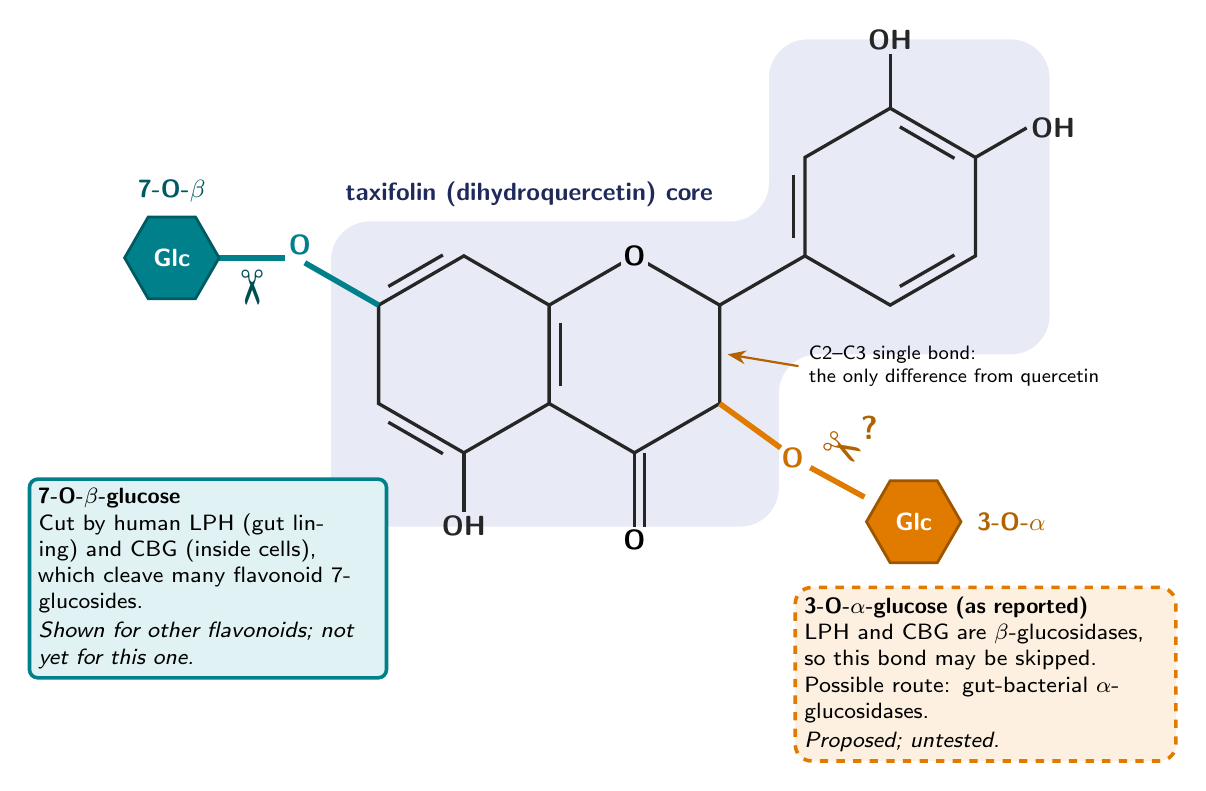
\begin{tikzpicture}[scale=1.25, font=\sffamily, bond/.style={line width=1.2pt, black!85}]
% ring A centre (0,0), ring C centre (1.732,0), pointy-top hexagons, side 1
\coordinate (C8) at (0,1); \coordinate (C8a) at (0.866,0.5); \coordinate (C4a) at (0.866,-0.5);
\coordinate (C5) at (0,-1); \coordinate (C6) at (-0.866,-0.5); \coordinate (C7) at (-0.866,0.5);
\coordinate (O1) at (1.732,1); \coordinate (C2) at (2.598,0.5); \coordinate (C3) at (2.598,-0.5); \coordinate (C4) at (1.732,-1);
\coordinate (C1p) at (3.464,1); \coordinate (C2p) at (3.464,2); \coordinate (C3p) at (4.33,2.5);
\coordinate (C4p) at (5.196,2); \coordinate (C5p) at (5.196,1); \coordinate (C6p) at (4.33,0.5);
% taxifolin core highlight
\fill[navylight, rounded corners=14pt] (-1.35,-1.75) -- (-1.35,1.35) -- (3.1,1.35) -- (3.1,3.2) -- (5.95,3.2) -- (5.95,0.0) -- (3.2,0.0) -- (3.2,-1.75) -- cycle;
\node[navy, font=\sffamily\bfseries\small, anchor=south west] at (-1.3,1.4) {taxifolin (dihydroquercetin) core};
% ring bonds
\draw[bond] (C8)--(C8a)--(C4a)--(C5)--(C6)--(C7)--cycle;
\draw[bond] (C8a)--(O1)--(C2)--(C3)--(C4)--(C4a);
\draw[bond] (C2)--(C1p);
\draw[bond] (C1p)--(C2p)--(C3p)--(C4p)--(C5p)--(C6p)--cycle;
% aromatic inner double bonds
\draw[bond] ($(C4a)!0.18!(C8a)!0.14!-90:(C8a)$) -- ($(C8a)!0.18!(C4a)!0.14!90:(C4a)$);
\draw[bond] ($(C8)!0.18!(C7)!0.14!-90:(C7)$) -- ($(C7)!0.18!(C8)!0.14!90:(C8)$);
\draw[bond] ($(C6)!0.18!(C5)!0.14!-90:(C5)$) -- ($(C5)!0.18!(C6)!0.14!90:(C6)$);
\draw[bond] ($(C1p)!0.18!(C2p)!0.14!90:(C2p)$) -- ($(C2p)!0.18!(C1p)!0.14!-90:(C1p)$);
\draw[bond] ($(C3p)!0.18!(C4p)!0.14!-90:(C4p)$) -- ($(C4p)!0.18!(C3p)!0.14!90:(C3p)$);
\draw[bond] ($(C5p)!0.18!(C6p)!0.14!-90:(C6p)$) -- ($(C6p)!0.18!(C5p)!0.14!90:(C5p)$);
% ring O label
\node[fill=navylight, inner sep=1pt, font=\sffamily\bfseries] at (O1) {O};
% C4 carbonyl, 5-OH, 3',4'-OH
\draw[bond] (C4) -- ++(0,-0.75) coordinate (O4); \draw[bond] ($(C4)+(0.1,0)$) -- ++(0,-0.75);
\node[below, inner sep=1pt, font=\sffamily\bfseries] at (O4) {O};
\draw[bond] (C5) -- ++(0,-0.6) node[below, inner sep=1pt, font=\sffamily\bfseries] {OH};
\draw[bond] (C3p) -- ++(0,0.55) node[above, inner sep=1pt, font=\sffamily\bfseries] {OH};
\draw[bond] (C4p) -- ++(0.52,0.3) node[right, inner sep=1pt, font=\sffamily\bfseries] {OH};
% single C2-C3 bond callout
\draw[orange!80!black, line width=0.8pt, -{Stealth}] (3.4,-0.12) node[right, font=\sffamily\scriptsize, align=left, text=black] {C2--C3 single bond:\\the only difference from quercetin} -- ($(C2)!0.5!(C3)+(0.08,0)$);
% 7-O-beta glucose (teal)
\draw[teal, line width=2pt] (C7) -- ++(-0.75,0.43) coordinate (O7);
\node[teal, font=\sffamily\bfseries] at ($(O7)+(-0.05,0.18)$) {O};
\draw[teal, line width=2pt] ($(O7)+(-0.2,0.05)$) -- ++(-0.7,0) coordinate (G7);
\node[regular polygon, regular polygon sides=6, minimum size=12mm, draw=teal!70!black, fill=teal, line width=1pt, text=white, font=\sffamily\bfseries\small] (g7) at ($(G7)+(-0.45,0)$) {Glc};
\node[teal!70!black, font=\sffamily\bfseries\small] at ($(g7.north)+(0,0.25)$) {7-O-$\beta$};
\node[font=\Large, teal!60!black, rotate=-90] at ($(O7)+(-0.55,-0.25)$) {\cut};
% 3-O-alpha glucose (orange)
\draw[orange, line width=2pt] (C3) -- ++(0.62,-0.45) coordinate (O3);
\node[orange!90!black, font=\sffamily\bfseries] at ($(O3)+(0.12,-0.1)$) {O};
\draw[orange, line width=2pt] ($(O3)+(0.3,-0.2)$) -- ++(0.55,-0.3) coordinate (G3);
\node[regular polygon, regular polygon sides=6, minimum size=12mm, draw=orange!70!black, fill=orange, line width=1pt, text=white, font=\sffamily\bfseries\small] (g3) at ($(G3)+(0.5,-0.25)$) {Glc};
\node[orange!80!black, font=\sffamily\bfseries\small, anchor=west] at ($(g3.east)+(0.05,0)$) {3-O-$\alpha$};
\node[font=\Large, orange!80!black, rotate=-30] at ($(O3)+(0.62,-0.02)$) {\cut};
\node[font=\sffamily\bfseries\large, orange!80!black] at ($(O3)+(0.9,0.2)$) {?};
% annotation boxes
\node[est, text width=4.3cm, font=\sffamily\footnotesize, align=left, anchor=north] at (-2.6,-1.25) {\textbf{7-O-$\beta$-glucose}\\ Cut by human LPH (gut lining) and CBG (inside cells), which cleave many flavonoid 7-glucosides.\\[1pt]\textit{Shown for other flavonoids; not yet for this one.}};
\node[prop, text width=4.6cm, font=\sffamily\footnotesize, align=left, anchor=north] at (5.3,-2.35) {\textbf{3-O-$\alpha$-glucose (as reported)}\\ LPH and CBG are \emph{$\beta$}-glucosidases, so this bond may be skipped. Possible route: gut-bacterial $\alpha$-glucosidases.\\[1pt]\textit{Proposed; untested.}};
\end{tikzpicture}
\end{adjustbox}\\[4pt]
\evlegend
\caption{The key compound as tentatively identified in the isolation paper~\cite{prasad2005}: \DQG. The taxifolin core is shaded. Scissors mark the two sugar bonds. The 7-\emph{O}-$\beta$ bond is the kind human LPH and CBG cut in other flavonoids~\cite{day1998}. The 3-\emph{O}-$\alpha$ bond may not be, which is why it carries a question mark. Stereochemistry is not shown.}
\label{fig:compound}
\end{figure}

\begin{figure}[tbp]
\centering
\begin{adjustbox}{max width=\linewidth}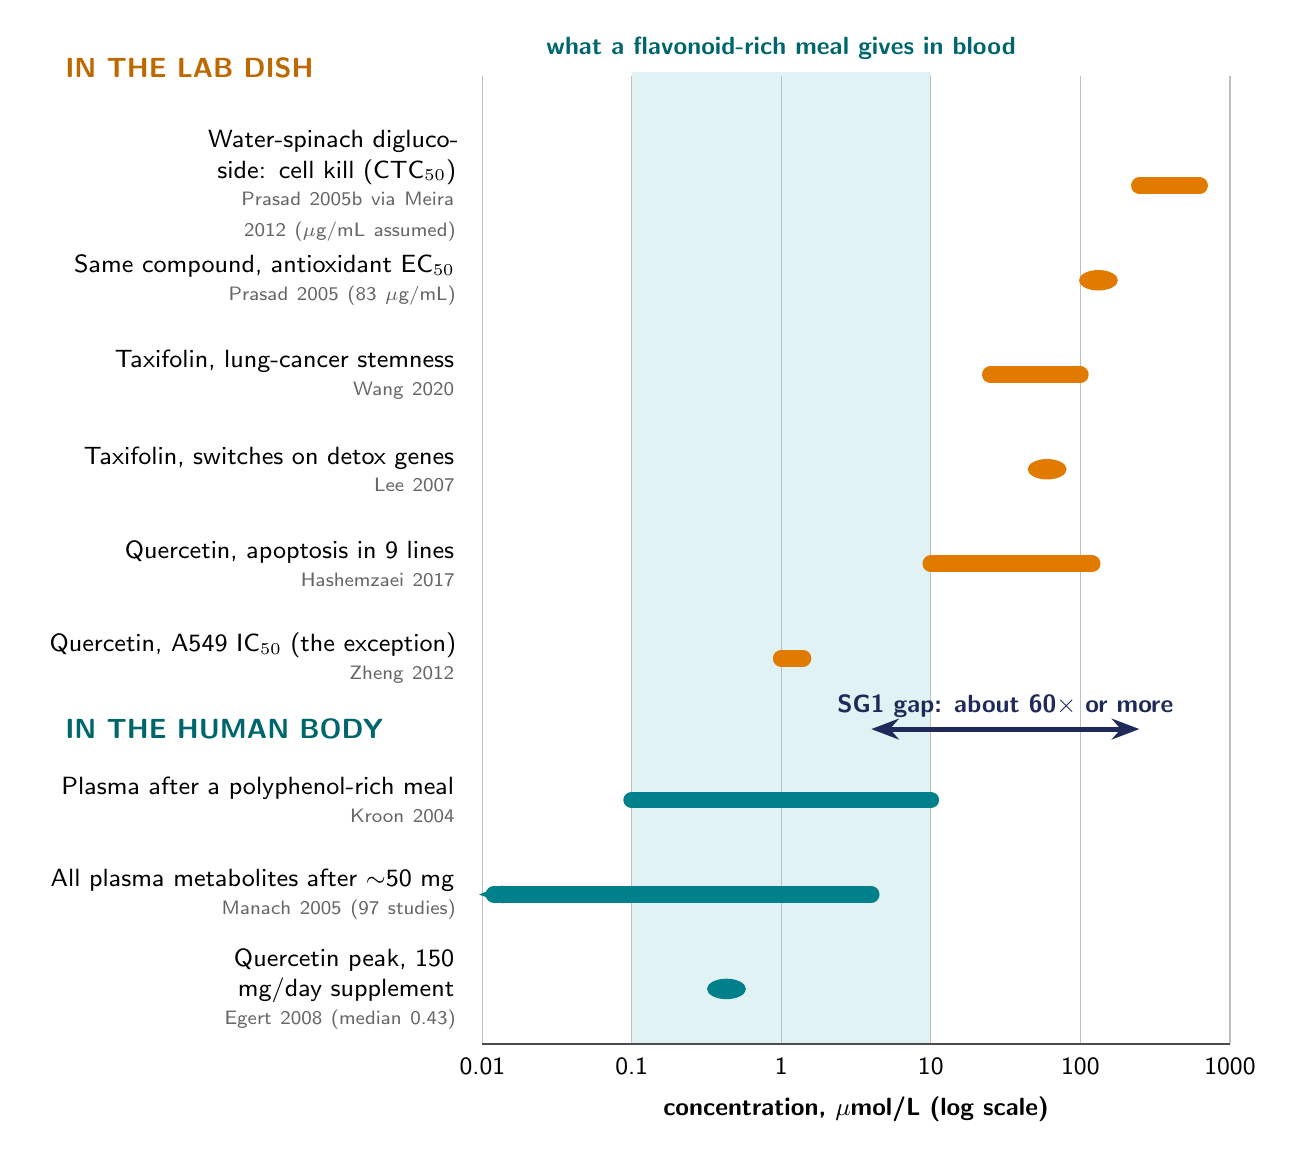
\begin{tikzpicture}[font=\sffamily, x=1.9cm, y=1cm]
% x = log10(concentration in micromolar) + 2 ; 0.01 uM -> 0, 1000 uM -> 5
\pgfmathsetmacro{\lg}{1}
\newcommand{\X}[1]{{log10(#1)+2}}
% achievable band 0.1-10 uM
\fill[teallight] ({log10(0.1)+2},0.45) rectangle ({log10(10)+2},-11.9);
\node[font=\sffamily\bfseries\small, text=teal!80!black, align=center] at ({log10(1)+2},0.75) {what a flavonoid-rich meal gives in blood};
% grid & axis
\foreach \v/\t in {0.01/0.01,0.1/0.1,1/1,10/10,100/100,1000/1000}{
  \draw[black!25] ({log10(\v)+2},0.4) -- ({log10(\v)+2},-11.9);
  \node[font=\sffamily\small, anchor=north] at ({log10(\v)+2},-11.95) {\t};}
\draw[line width=1pt, black!70] (0,-11.9) -- (5,-11.9);
\node[font=\sffamily\small\bfseries, anchor=north] at (2.5,-12.45) {concentration, $\mu$mol/L (log scale)};
% row macro: y, lo, hi, colour, label, source
\newcommand{\rng}[6]{%
  \draw[line width=6pt, #4, line cap=round] ({log10(#2)+2},#1) -- ({log10(#3)+2},#1);
  \node[anchor=east, font=\sffamily\small, text width=5.3cm, align=right] at (-0.12,#1) {#5\\[-1pt]{\scriptsize\color{black!60}#6}};}
\newcommand{\pt}[5]{%
  \fill[#3] ({log10(#2)+2},#1) circle (0.13);
  \node[anchor=east, font=\sffamily\small, text width=5.3cm, align=right] at (-0.12,#1) {#4\\[-1pt]{\scriptsize\color{black!60}#5}};}
\node[anchor=west, font=\sffamily\bfseries, text=orange!85!black] at (-2.85,0.5) {IN THE LAB DISH};
\rng{-1.0}{248}{627}{orange}{Water-spinach diglucoside: cell kill (CTC$_{50}$)}{Prasad 2005b via Meira 2012 ($\mu$g/mL assumed)}
\pt{-2.2}{132}{orange}{Same compound, antioxidant EC$_{50}$}{Prasad 2005 (83 $\mu$g/mL)}
\rng{-3.4}{25}{100}{orange}{Taxifolin, lung-cancer stemness}{Wang 2020}
\pt{-4.6}{60}{orange}{Taxifolin, switches on detox genes}{Lee 2007}
\rng{-5.8}{10}{120}{orange}{Quercetin, apoptosis in 9 lines}{Hashemzaei 2017}
\rng{-7.0}{1.0}{1.4}{orange}{Quercetin, A549 IC$_{50}$ (the exception)}{Zheng 2012}
\node[anchor=west, font=\sffamily\bfseries, text=teal!80!black] at (-2.85,-7.9) {IN THE HUMAN BODY};
\rng{-8.8}{0.1}{10}{teal}{Plasma after a polyphenol-rich meal}{Kroon 2004}
\draw[line width=6pt, teal, line cap=round] ({log10(0.012)+2},-10.0) -- ({log10(4)+2},-10.0);
\draw[teal, line width=1.5pt, -{Stealth[length=3mm]}] ({log10(0.02)+2},-10.0) -- (-0.02,-10.0);
\node[anchor=east, font=\sffamily\small, text width=5.3cm, align=right] at (-0.12,-10.0) {All plasma metabolites after $\sim$50 mg\\[-1pt]{\scriptsize\color{black!60}Manach 2005 (97 studies)}};
\pt{-11.2}{0.431}{teal}{Quercetin peak, 150 mg/day supplement}{Egert 2008 (median 0.43)}
% gap arrow
\draw[{Stealth[length=3.5mm]}-{Stealth[length=3.5mm]}, line width=1.8pt, navy] ({log10(4)+2},-7.9) -- ({log10(248)+2},-7.9) node[midway, above, font=\sffamily\bfseries\small, text=navy] {SG1 gap: about 60$\times$ or more};
\end{tikzpicture}
\end{adjustbox}
\caption{The dose gap (SG1), on a log scale in $\mu$mol/L. Orange bars and dots are concentrations used in the laboratory; teal ones are what people actually reach in blood. Each value comes from the source named under its label. The diglucoside values convert the reported CTC$_{50}$ and EC$_{50}$ from $\mu$g/mL to $\mu$M using a molar mass of about 628~g/mol, on the assumption that ``mg/mL'' in the review is a misprint for $\mu$g/mL~\cite{prasad2005b,meira2012}. The merromoside IC$_{50}$ (182.8~$\mu$g/mL~\cite{sasikala2022}) is not plotted because its molar mass is not given in our sources.}
\label{fig:dose}
\end{figure}

\begin{figure}[tbp]
\centering
\begin{adjustbox}{max width=\linewidth}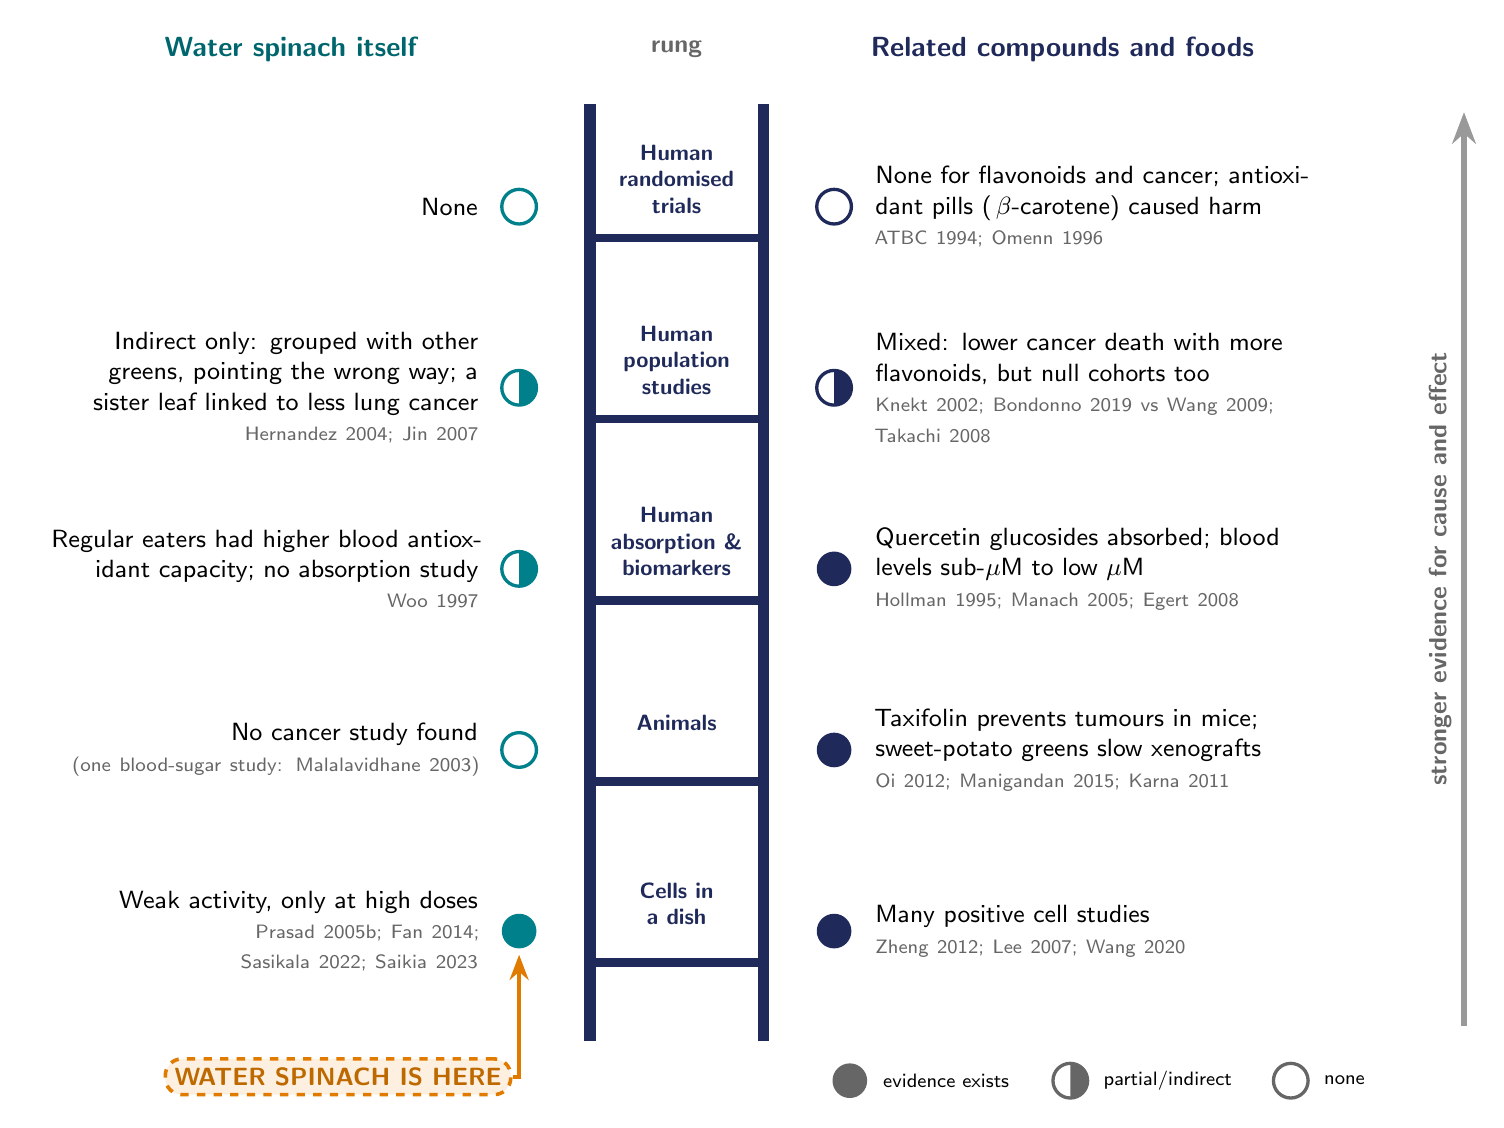
\begin{tikzpicture}[font=\sffamily, x=1cm, y=1cm]
\newcommand{\full}[1]{\fill[#1] (0,0) circle (0.22);}
\newcommand{\half}[1]{\draw[#1, line width=1.2pt] (0,0) circle (0.22); \fill[#1] (0,-0.22) arc[start angle=-90,end angle=90,radius=0.22] -- cycle;}
\newcommand{\none}[1]{\draw[#1, line width=1.2pt] (0,0) circle (0.22);}
% ladder rails and rungs
\draw[navy, line width=4pt] (-1.1,-0.6) -- (-1.1,11.3); \draw[navy, line width=4pt] (1.1,-0.6) -- (1.1,11.3);
\foreach \i/\t/\ic in {0/{Cells in\\ a dish}/flask,1/{Animals}/mouse,2/{Human\\ absorption \&\\ biomarkers}/people,3/{Human\\ population\\ studies}/people,4/{Human\\ randomised\\ trials}/people}{
  \draw[navy, line width=3pt] (-1.1,\i*2.3+0.4) -- (1.1,\i*2.3+0.4);
  \node[font=\sffamily\bfseries\footnotesize, align=center, text=navy, fill=white, inner sep=1.5pt] at (0,\i*2.3+1.15) {\t};
}
% column headers
\node[font=\sffamily\bfseries, text=teal!80!black] at (-4.9,12.0) {Water spinach itself};
\node[font=\sffamily\bfseries, text=navy] at (4.9,12.0) {Related compounds and foods};
\node[font=\sffamily\bfseries\small, text=black!60] at (0,12.0) {rung};
% cell macro: x-side (L/R), rung index, marker, colour, text
\newcommand{\cellL}[3]{\begin{scope}[shift={(-2.0,#1*2.3+0.8)}]#2\end{scope}\node[anchor=east, text width=5.6cm, align=right, font=\sffamily\small] at (-2.4,#1*2.3+0.8) {#3};}
\newcommand{\cellR}[3]{\begin{scope}[shift={(2.0,#1*2.3+0.8)}]#2\end{scope}\node[anchor=west, text width=5.6cm, align=left, font=\sffamily\small] at (2.4,#1*2.3+0.8) {#3};}
\cellL{0}{\full{teal}}{Weak activity, only at high doses\\{\scriptsize\color{black!60}Prasad 2005b; Fan 2014; Sasikala 2022; Saikia 2023}}
\cellR{0}{\full{navy}}{Many positive cell studies\\{\scriptsize\color{black!60}Zheng 2012; Lee 2007; Wang 2020}}
\cellL{1}{\none{teal}}{No cancer study found\\{\scriptsize\color{black!60}(one blood-sugar study: Malalavidhane 2003)}}
\cellR{1}{\full{navy}}{Taxifolin prevents tumours in mice; sweet-potato greens slow xenografts\\{\scriptsize\color{black!60}Oi 2012; Manigandan 2015; Karna 2011}}
\cellL{2}{\half{teal}}{Regular eaters had higher blood antioxidant capacity; no absorption study\\{\scriptsize\color{black!60}Woo 1997}}
\cellR{2}{\full{navy}}{Quercetin glucosides absorbed; blood levels sub-$\mu$M to low $\mu$M\\{\scriptsize\color{black!60}Hollman 1995; Manach 2005; Egert 2008}}
\cellL{3}{\half{teal}}{Indirect only: grouped with other greens, pointing the wrong way; a sister leaf linked to less lung cancer\\{\scriptsize\color{black!60}Hernandez 2004; Jin 2007}}
\cellR{3}{\half{navy}}{Mixed: lower cancer death with more flavonoids, but null cohorts too\\{\scriptsize\color{black!60}Knekt 2002; Bondonno 2019 vs Wang 2009; Takachi 2008}}
\cellL{4}{\none{teal}}{None}
\cellR{4}{\none{navy}}{None for flavonoids and cancer; antioxidant pills (\,$\beta$-carotene) caused harm\\{\scriptsize\color{black!60}ATBC 1994; Omenn 1996}}
% you-are-here
\node[prop, font=\sffamily\bfseries\small, text=orange!85!black, align=center] (here) at (-4.3,-1.05) {WATER SPINACH IS HERE};
\draw[aprop, solid] (here.east) -| (-2.0,0.5);
% strength arrow
\draw[-{Stealth[length=4mm]}, line width=2.5pt, black!40] (10.0,-0.4) -- (10.0,11.2) node[midway, rotate=90, above, font=\sffamily\bfseries\small, text=black!60] {stronger evidence for cause and effect};
% key
\begin{scope}[shift={(2.2,-1.1)}]
\full{black!60} \node[anchor=west, font=\sffamily\scriptsize] at (0.3,0) {evidence exists};
\begin{scope}[shift={(2.8,0)}]\half{black!60}\end{scope} \node[anchor=west, font=\sffamily\scriptsize] at (3.1,0) {partial/indirect};
\begin{scope}[shift={(5.6,0)}]\none{black!60}\end{scope} \node[anchor=west, font=\sffamily\scriptsize] at (5.9,0) {none};
\end{scope}
\end{tikzpicture}
\end{adjustbox}
\caption{The evidence ladder. Rungs rise from cell studies to randomised human trials. Left: evidence about water spinach itself. Right: evidence about its related compounds and foods (taxifolin, quercetin, flavonoids, vegetables, sweet-potato greens). Water spinach sits on the bottom rung, with only indirect hints above it, and nothing yet at the trial rung. Sources are named under each entry.}
\label{fig:ladder}
\end{figure}

\subsection{Stop-gap wording}

\begin{sgbox}{SG1 · Dose / Bioavailability}
In-vitro concentrations (low to high micromolar, or tens to hundreds of $\mu$g/mL for extracts) are approached only in attenuated, chronic form, by repeated dietary exposure to aglycone metabolites released by LPH/CBG deglycosylation or by colonic bacteria, never by a single meal reaching laboratory concentrations.
\end{sgbox}

\noindent\emph{Why it is a bridge, not a proof.} After about 50~mg of aglycone equivalents, human plasma polyphenol metabolites reach at most about 4~$\mu$M~\cite{manach2005}, and a polyphenol-rich meal gives about 0.1--10~$\mu$M~\cite{kroon2004}. Even 150~mg/day of quercetin as a supplement gives a median peak of 0.43~$\mu$M~\cite{egert2008}. Most antiproliferative concentrations in the cited cell studies are 10--120~$\mu$M~\cite{hashemzaei2017,wang2020,hisaka2020}, and the water-spinach diglucoside was cytotoxic only at roughly 250--630~$\mu$M~\cite{prasad2005b} (Figure~\ref{fig:dose}). Free taxifolin is poorly bioavailable in rats (0.49\%~\cite{yang2016}), as is a taxifolin 3-glycoside (about 1.2\%~\cite{shi2020}). Quercetin in A549 cells (IC$_{50}$ about 1~$\mu$M~\cite{zheng2012}) is an exception, not the rule. SG1 therefore does not claim equivalence of dose. It claims that low, repeated exposure over years is the relevant scale, that high consumers really do take in hundreds of milligrams of polyphenols a day, much of it from this plant~\cite{thu2004}, and that phase-II induction by taxifolin~\cite{lee2007} is the kind of mechanism that could act at such exposures. The first author's own framing was persistence (``persistent cytotoxicity would result in an overall greater at poptosis towards cancer cell lines,'' Section~\ref{sec:commentary}). Our reading is that persistence of \emph{gene induction}, not of cell killing, is the more plausible version. The $\alpha$-link caveat sits inside SG1: if human $\beta$-glucosidases cannot cut the 3-\emph{O}-$\alpha$ bond~\cite{day1998,prasad2005}, release of taxifolin falls to colonic bacteria~\cite{braune2001}. Human data on an $\alpha$-glucosylated quercetin glucoside show that $\alpha$-sugars need not block absorption~\cite{murota2010}.

\begin{sgbox}{SG2 · Cross-species / model homology}
Responses of cancer cell lines and rodents (together with the LPH evidence obtained from sheep enzyme and rat intestine) map onto human tissue responses by homology of molecular targets and of the deglycosylation enzymes.
\end{sgbox}

\noindent\emph{Why it is a bridge, not a proof.} The first author asked exactly this question in the thread (quoted in Section~\ref{sec:mechanism}). The enzyme side of the homology is comparatively strong. LPH characterised from sheep~\cite{day2000} and LPH-dependent absorption in rat jejunum~\cite{day2003} mirror the human enzymes~\cite{nemeth2003}. The target side (EGFR/PI3K, Nrf2/ARE, Wnt/$\beta$-catenin) is conserved, but chemically induced tumours in mice are not human carcinogenesis~\cite{oi2012,manigandan2015}, and xenografts are models of treatment, not prevention~\cite{karna2011,zheng2012}.

\begin{sgbox}{SG3 · Prevention vs Cure}
What diet can plausibly contribute is a modest preventive tendency, a slightly lower risk over years, not the treatment or cure of established cancer (cure remains unshown and is not claimed).
\end{sgbox}

\noindent\emph{Why it is a bridge, not a proof.} Cohort data show small inverse associations for flavonoids and vegetables~\cite{knekt2002,aune2017,bondonno2019,parmenter2025}, but other cohorts, a Mendelian randomisation and two systematic reviews are null or inconclusive~\cite{wang2009,takachi2008,wei2024,grosso2017,jin2012}. Theory suggests that small, persistent growth reductions are what matter for prevention~\cite{akhmetzhanov2014}. Pharmacological cytotoxicity from the same genus did not become a cure~\cite{kasturi1998}, and antioxidant supplements given to prevent cancer caused harm~\cite{alphatocopherolbetac1994,omenn1996,klein2011}.

% =====================================================================
\section{Proposed Mechanism}
\label{sec:mechanism}

\begin{voicebox}
This section is written in my voice, as the first author. The mechanism below is my proposal; the labels say how much of it is known.
\end{voicebox}

My questions to Grok on 24 September were really one question asked in five pieces. I wanted to see the molecule, to know whether it would clump together, which of our enzymes would free the active part, and whether other animals would do the same. Here are those questions as I asked them, and what the literature says about each.

\paragraph{The molecule.}
\BQ{2103095356758315034}

\noindent The core I wanted highlighted is actually \emph{dihydro}quercetin, taxifolin, not quercetin. It lacks one double bond, and that changes its biology: it is a weaker VEGF inhibitor~\cite{luo2008}, and unlike quercetin it was not mutagenic in the Ames test~\cite{bjeldanes1977}. Figure~\ref{fig:compound} draws it with both sugars. I also said at the time:

\BQ{2103100421565034781}

\noindent The literature does support a ``broad'' effect in the sense of several pathways at once (M6--M9 below). But every one of them has been shown only in cells or animals.

\paragraph{Polymerisation.}
\BQ{2103097209789227371}

\noindent We found no report that this diglucoside polymerises. Grok's reply, that free taxifolin can form oligomers under oxidative enzymes and that the sugars block the key sites, was not checked against a primary source, and I do not rely on it.

\paragraph{The enzymes.}
\BQ{2103097586647503177}

\noindent For glucose attached by a $\beta$-bond, the answer is LPH on the gut lining and CBG inside cells~\cite{day1998,day2000,nemeth2003}. The catch is that the isolation paper reports the 3-position sugar as $\alpha$-linked~\cite{prasad2005}. If so, it probably needs a different enzyme, possibly from gut bacteria. This is step M3, and I treat it as the single most important unknown.

\paragraph{Other mammals.}
\BQ{2103098371632455790}

\noindent Yes for the enzyme class. The key LPH work used sheep enzyme~\cite{day2000} and rat intestine~\cite{day2003}. That is why the animal feeding study in Section~\ref{sec:animal} is a fair test, and why SG2 is still needed to carry its result to people.

\paragraph{The proposed path, step by step.} Table~\ref{tab:mech} walks from the leaf to a lower cancer risk. Each step is labelled \tagE{} (human data or human-tissue biochemistry), \tagM{} (cells or animals) or \tagP{} (my proposal), and mapped to the experiment in Section~\ref{sec:studies} that would test it. Figure~\ref{fig:mechanism} draws the same path inside a cell.

{\small\sloppy
\renewcommand{\arraystretch}{1.3}
\begin{longtable}{@{}>{\raggedright\arraybackslash}p{0.85cm} >{\raggedright\arraybackslash}p{5.95cm} >{\raggedright\arraybackslash}p{3.2cm} >{\raggedright\arraybackslash}p{4.5cm}@{}}
\caption{The proposed mechanism, with evidence labels and the experiment that tests each step.}\label{tab:mech}\\
\toprule
\textbf{Step} & \textbf{What happens} & \textbf{Label and source} & \textbf{Tested by}\\
\midrule\endfirsthead
\toprule
\textbf{Step} & \textbf{What happens} & \textbf{Label and source} & \textbf{Tested by}\\
\midrule\endhead
\bottomrule\endfoot
\rowcolor{teallight} M1 & Water-spinach leaves contain flavonoid glycosides, including a tentatively identified taxifolin 3,7-diglucoside. & \tagE~\cite{prasad2005,hefnygad2018,saikia2023}; diglucoside not found by~\cite{lawal2016} & Step~0: NMR and quantification in raw and cooked leaves from several cultivars\\
\rowcolor{teallight} M2 & LPH (gut lining) and CBG (inside cells) cut the 7-\emph{O}-$\beta$ glucose. & \tagE{} for flavonoid 7-glucosides~\cite{day1998,nemeth2003}; \tagP{} for this compound & Step~0: incubate with human LPH, CBG and small-intestinal extract\\
\rowcolor{orangelight} M3 & The 3-\emph{O}-$\alpha$ glucose is cut by gut-bacterial (or other) $\alpha$-glucosidases; bacteria may also degrade taxifolin to phenolic acids. & \tagP; related: \cite{murota2010} (humans), \cite{braune2001} (bacteria, \emph{in vitro}) & Step~0 stool-slurry assay; microbiome arm of the animal study\\
\rowcolor{navylight} M4 & Taxifolin enters gut-lining cells; intact glycosides are not carried by SGLT1. & \tagM: rat F 0.49\%~\cite{yang2016}, astilbin 1.2\%~\cite{shi2020}; \cite{kottra2007} & Step~1 meal study; animal plasma levels\\
\rowcolor{teallight} M5 & Liver and gut conjugate it (glucuronide, sulfate, methyl); low-$\mu$M conjugates circulate. & \tagE{} for polyphenols~\cite{kroon2004,manach2005}; \tagP{} for taxifolin from this food & Step~1: LC-MS/MS of plasma and urine, with and without deconjugation\\
\rowcolor{navylight} M6 & Taxifolin binds and inhibits EGFR and PI3K, damping growth signals. & \tagM~\cite{oi2012} (topical, mouse skin) & Animal study: tumour number and size; tissue phospho-EGFR/Akt as secondary markers\\
\rowcolor{navylight} M7 & Taxifolin switches on Nrf2 and antioxidant-response-element genes (\emph{NQO1}, \emph{GST}). & \tagM~\cite{lee2007,manigandan2015} & Animal study: colon NQO1 activity; human biomarker substudy\\
\rowcolor{navylight} M8 & Taxifolin lowers NF-$\kappa$B and Wnt/$\beta$-catenin signalling (COX-2, cyclin~D1) and cancer-cell stemness. & \tagM~\cite{manigandan2015,wang2020} & Animal study: tumour histology and these markers\\
\rowcolor{navylight} M9 & The glycosides and extracts scavenge radicals and protect DNA. & \tagM~\cite{prasad2005,saikia2023}; caution:~\cite{bjelakovic2012} & Human substudy: oxidative-DNA-damage markers by intake\\
\rowcolor{orangelight} M10 & Over years, fewer mutations and less growth signalling mean a slightly lower cancer risk. & \tagP; related:~\cite{bondonno2019,akhmetzhanov2014} & Animal tumour endpoints; cross-sectional and cohort studies\\
\rowcolor{navylight} Side\newline route & \emph{In the pan}: water-spinach polyphenols inhibit carcinogenic heterocyclic amines forming in grilled meat, with no absorption needed. & \tagM~\cite{huang2026} (food chemistry) & Cooking study measuring heterocyclic amines with and without the vegetable\\
\end{longtable}
}

\begin{figure}[H]
\centering
\begin{adjustbox}{max width=\linewidth}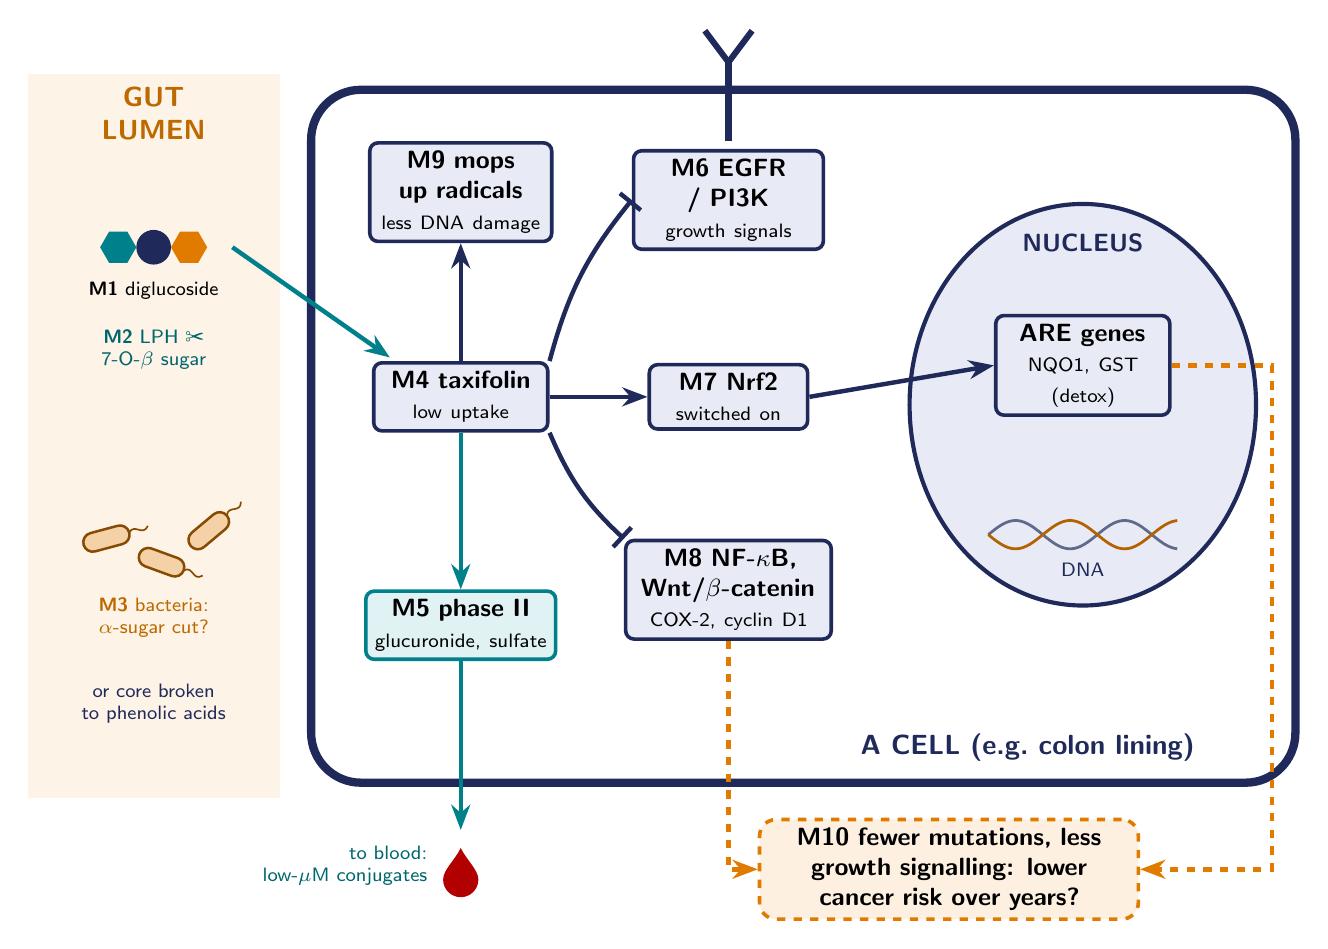
\begin{tikzpicture}[font=\sffamily\small, x=1cm, y=1cm,
  bx/.style={inner sep=3pt, align=center, font=\sffamily\small, text width=#1},
  bx/.default=2.4cm]
% ---- lumen ----
\fill[orangelight!80] (-1.5,-4.6) rectangle (1.7,4.6);
\node[font=\sffamily\bfseries, text=orange!85!black, align=center] at (0.1,4.1) {GUT\\LUMEN};
\fill[navy] (0.1,2.4) circle (0.22);
\node[regular polygon, regular polygon sides=6, minimum size=4.6mm, inner sep=0pt, fill=teal] at (-0.35,2.4) {};
\node[regular polygon, regular polygon sides=6, minimum size=4.6mm, inner sep=0pt, fill=orange] at (0.55,2.4) {};
\node[font=\sffamily\scriptsize, align=center] at (0.1,1.85) {\textbf{M1} diglucoside};
\node[font=\sffamily\scriptsize, align=center, text=teal!80!black] at (0.1,1.1) {\textbf{M2} LPH \cut\\ 7-O-$\beta$ sugar};
\foreach \dx/\dy/\r in {-0.6/-1.3/15,0.1/-1.6/-20,0.7/-1.2/40}{\pic[rotate=\r] at ({0.1+\dx},{\dy}) {bug};}
\node[font=\sffamily\scriptsize, align=center, text=orange!85!black] at (0.1,-2.3) {\textbf{M3} bacteria:\\ $\alpha$-sugar cut?};
\node[font=\sffamily\scriptsize, align=center, text=navy] at (0.1,-3.4) {or core broken\\ to phenolic acids};
% ---- cell ----
\draw[navy, line width=3pt, fill=white, rounded corners=18pt] (2.1,-4.4) rectangle (14.6,4.4);
\node[font=\sffamily\bfseries, text=navy] at (11.2,-3.95) {A CELL (e.g.\ colon lining)};
\draw[navy, line width=1.5pt, fill=navylight] (11.9,0.4) ellipse (2.2 and 2.55);
\node[font=\sffamily\bfseries\small, text=navy] at (11.9,2.45) {NUCLEUS};
\draw[navy!70, line width=1pt, domain=0:2.4, samples=60, smooth, variable=\t] plot ({10.7+\t},{-1.25+0.18*sin(\t*260)});
\draw[orange!80!black, line width=1pt, domain=0:2.4, samples=60, smooth, variable=\t] plot ({10.7+\t},{-1.25-0.18*sin(\t*260)});
\node[font=\sffamily\scriptsize, text=navy] at (11.9,-1.7) {DNA};
% taxifolin
\draw[aest] (1.1,2.4) -- (3.1,1.0);
\node[mod, bx=2.0cm] (tax) at (4.0,0.5) {\textbf{M4 taxifolin}\\{\scriptsize low uptake}};
\node[est, bx=2.2cm] (p2) at (4.0,-2.4) {\textbf{M5 phase II}\\{\scriptsize glucuronide, sulfate}};
\draw[aest] (tax) -- (p2);
\draw[aest] (p2.south) -- (4.0,-5.0);
\pic[scale=0.8] at (4.0,-5.55) {blood};
\node[font=\sffamily\scriptsize, text=teal!80!black, anchor=east, align=right] at (3.7,-5.45) {to blood:\\ low-$\mu$M conjugates};
% EGFR
\draw[navy, line width=2.2pt] (7.4,4.75) -- (7.4,3.75); \draw[navy, line width=2.2pt] (7.4,4.75) -- (7.1,5.15); \draw[navy, line width=2.2pt] (7.4,4.75) -- (7.7,5.15);
\node[mod, bx=2.2cm] (egfr) at (7.4,3.0) {\textbf{M6 EGFR / PI3K}\\{\scriptsize growth signals}};
\draw[ainh] (tax.north east) to[bend left=12] (egfr.west);
% antioxidant
\node[mod, bx=2.1cm] (ros) at (4.0,3.1) {\textbf{M9 mops up radicals}\\{\scriptsize less DNA damage}};
\draw[amod] (tax.north) -- (ros.south);

% Nrf2
\node[mod, bx=1.8cm] (nrf) at (7.4,0.5) {\textbf{M7 Nrf2}\\{\scriptsize switched on}};
\draw[amod] (tax.east) -- (nrf.west);
\node[mod, bx=2.0cm] (are) at (11.9,0.9) {\textbf{ARE genes}\\{\scriptsize NQO1, GST (detox)}};
\draw[amod] (nrf.east) -- (are.west);
% NF-kB / Wnt
\node[mod, bx=2.4cm] (nfk) at (7.4,-1.95) {\textbf{M8 NF-$\kappa$B,}\\\textbf{Wnt/$\beta$-catenin}\\{\scriptsize COX-2, cyclin D1}};
\draw[ainh] (tax.south east) to[bend right=12] (nfk.north west);
% outcome below the cell
\node[prop, bx=4.6cm] (out) at (10.2,-5.5) {\textbf{M10 fewer mutations, less growth signalling: lower cancer risk over years?}};
\draw[aprop] (nfk.south) |- (out.west);
\draw[aprop] (are.east) -- (14.3,0.9) |- (out.east);
\end{tikzpicture}
\end{adjustbox}\\[4pt]
\evlegend
\caption{The proposed mechanism inside a cell, with steps M1--M10 as in Table~\ref{tab:mech}. Teal: established; navy: reported in cell or animal models; orange dashed: proposed. Bar-headed arrows mean inhibition. Only actions reported in the cited sources are drawn~\cite{lee2007,oi2012,manigandan2015,wang2020,prasad2005,saikia2023}.}
\label{fig:mechanism}
\end{figure}

\noindent The honest summary of my mechanism is this. The front end (M1, M2, M5) rests on solid human biochemistry, but has not yet been shown for this compound. The middle (M6--M9) is well supported in models, but at concentrations above what diet delivers. The end (M10) is my proposal. The weakest link is M3, the $\alpha$-sugar, which is why the study programme starts there.

% =====================================================================
\section{Counter-evidence and Limitations}
\label{sec:counter}

The thesis survives only if the evidence against it is stated as plainly as the evidence for it. The main points are listed here in rough order of weight.

\begin{enumerate}[label=\textbf{C\arabic*.}, leftmargin=2.4em]
\item \textbf{No water-spinach cancer data, and one signal the wrong way.} No cohort, case-control or trial has examined water-spinach intake and cancer. The only human cancer-related association we found that touches it is exploratory. In it, ``taro leaves/ong choy/marunggay'' as a lignan-source group was \emph{positively} associated with premalignant cervical lesions~\cite{hernandez2004}. The nearest favourable datum concerns sweet-potato leaves, not water spinach~\cite{jin2007}. The one water-spinach biomarker study measured antioxidant capacity, not cancer~\cite{woo1997}.
\item \textbf{The flavonoid and vegetable epidemiology is mixed.} Against the positive cohorts~\cite{knekt2002,bondonno2019,parmenter2025} stand null ones~\cite{wang2009,takachi2008}, inconclusive meta-analyses and systematic reviews~\cite{grosso2017,jin2012}, an umbrella review finding few strong diet-cancer associations~\cite{papadimitriou2021}, and a null Mendelian randomisation for vegetables and gastrointestinal cancers~\cite{wei2024}. Residual confounding by overall healthy lifestyle is a standing concern.
\item \textbf{``Antioxidant'' has a bad track record as a prevention mechanism.} $\beta$-Carotene and vitamin~E supplements increased cancer in large trials~\cite{alphatocopherolbetac1994,omenn1996,klein2011}, and antioxidant supplements do not lower mortality~\cite{bjelakovic2012}. M9 is therefore the least trustworthy mechanism step. The thesis must stay a food-level hypothesis.
\item \textbf{The dose gap is large.} Most positive cell studies used aglycones at 10--120~$\mu$M or more, against plasma levels of about 0.1--10~$\mu$M, mostly as conjugates~\cite{kroon2004,manach2005}. The diglucoside itself acted only at roughly 250--630~$\mu$M and without selectivity for cancer cells~\cite{prasad2005b}.
\item \textbf{Bioavailability of the core is poor, and bacteria may destroy it.} Oral taxifolin reached blood at 0.49\% in rats~\cite{yang2016}, a taxifolin 3-glycoside at about 1.2\%~\cite{shi2020}, and gut bacteria can degrade taxifolin to phenolic acids~\cite{braune2001}.
\item \textbf{The chemistry is uncertain.} The key compound was identified once, tentatively~\cite{prasad2005}, and a later LC-MS/MS survey of three cultivars did not report it~\cite{lawal2016}. Its C-3 linkage is $\alpha$ in the isolation paper and $\beta$ in the review~\cite{meira2012}. Any effect of water spinach may come from other constituents, such as quercetin glycosides~\cite{lawal2016,hefnygad2018}.
\item \textbf{The plant can carry carcinogens from its water.} Arsenic in water spinach from contaminated Guangzhou sites gave screening cancer risks of $2.2$--$4.1\times10^{-3}$~\cite{wu2026}. Mercury, cadmium and lead~\cite{gothberg2002}, nitrate~\cite{thang2021}, faecal pathogens~\cite{vuong2007} and flukes~\cite{graczyk2001} are documented in some settings, although wastewater-grown plants in Hanoi were mostly within limits~\cite{marcussen2008}. The first author's ``drainage ditches'' remark is a reason to specify clean sourcing, not a recommendation to forage there.
\item \textbf{Resin glycosides are a second, unassessed exposure.} The plant contains cytotoxic resin glycosides~\cite{fan2014,sasikala2022}. They appear to be heat-labile~\cite{toy2022}, which is reassuring for cooked greens but means their fate in the diet is unknown.
\item \textbf{Method limits of this paper.} The corpus was built by one search process over one day, weighted toward English-language, indexed sources. We did not read every full text, and several numbers come from abstracts. Section~\ref{sec:verification} documents the one case where a secondary source was needed.
\end{enumerate}

% =====================================================================
\section{Proposed Studies}
\label{sec:studies}

\begin{voicebox}
This section is written in my voice, as the first author. It is a design proposal, not a report of results. All numbers are labelled assumptions to be refined with pilot data and a statistician.
\end{voicebox}

I want these studies run in order, each one gating the next, so that no animal or large human study goes ahead before the cheap bench questions are answered. Figure~\ref{fig:studies} shows the programme.

\begin{figure}[H]
\centering
\begin{adjustbox}{max width=\linewidth}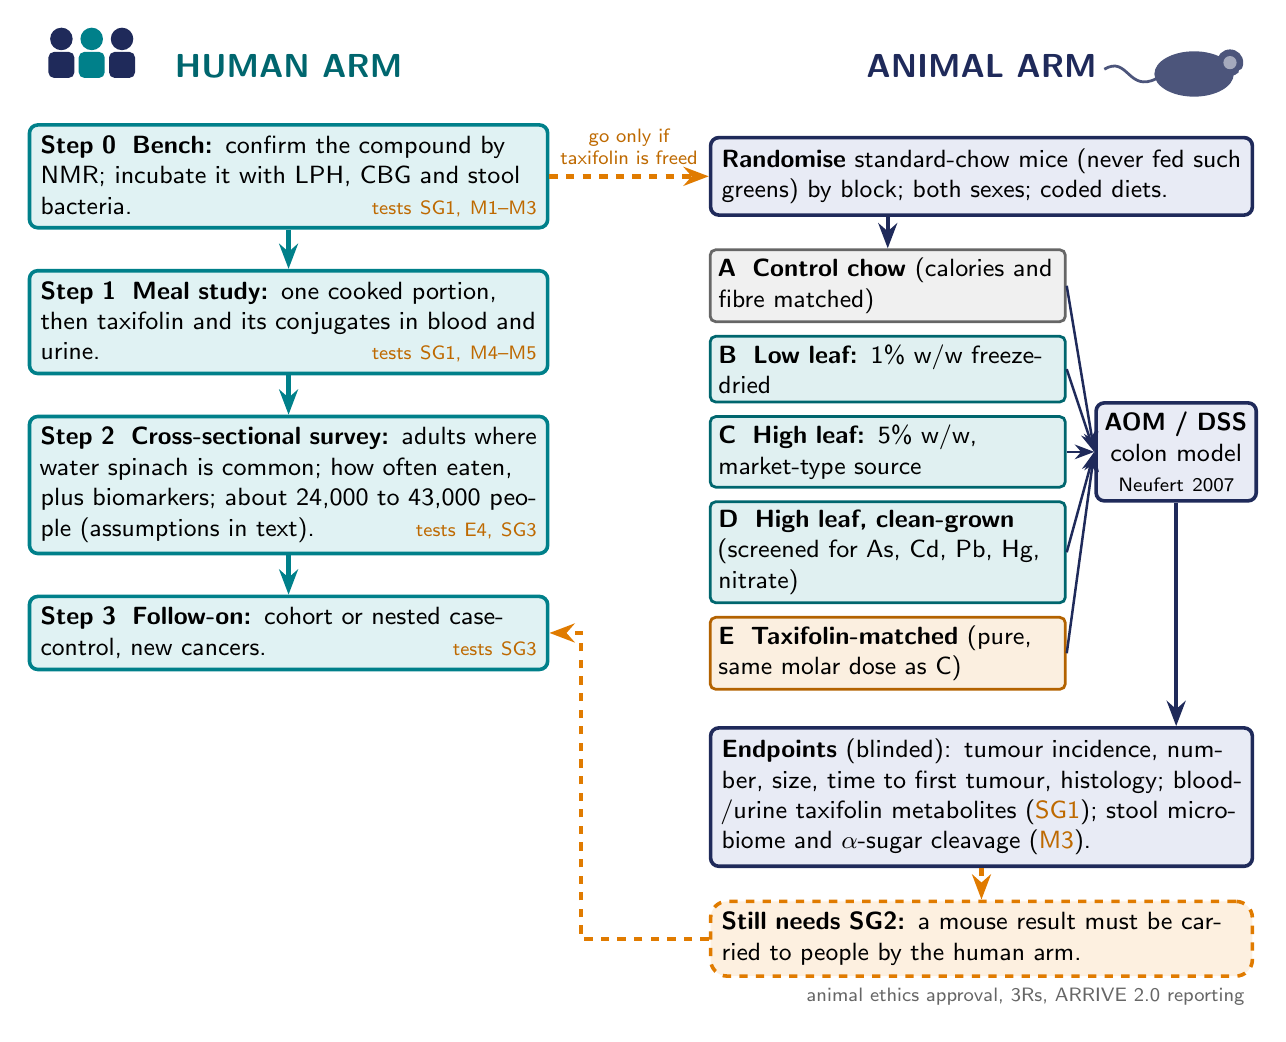
\begin{tikzpicture}[font=\sffamily\small, x=1cm, y=1cm,
  st/.style={text width=6.3cm, align=left, inner sep=4pt, font=\sffamily\small},
  arm/.style={text width=4.3cm, align=left, inner sep=3pt, font=\sffamily\small, rounded corners=2pt, draw=#1!80!black, line width=1pt, fill=#1!12}]
% ===== HUMAN ARM =====
\node[font=\sffamily\bfseries\large, text=teal!80!black] at (-4.0,0.4) {HUMAN ARM};
\pic[scale=1.1] at (-6.5,0.25) {people};
\node[st, est] (h0) at (-4.0,-1.0) {\textbf{Step 0 \;Bench:} confirm the compound by NMR; incubate it with LPH, CBG and stool bacteria.\hfill{\scriptsize\color{orange!85!black}tests SG1, M1--M3}};
\node[st, est, below=5mm of h0] (h1) {\textbf{Step 1 \;Meal study:} one cooked portion, then taxifolin and its conjugates in blood and urine.\hfill{\scriptsize\color{orange!85!black}tests SG1, M4--M5}};
\node[st, est, below=5mm of h1] (h2) {\textbf{Step 2 \;Cross-sectional survey:} adults where water spinach is common; how often eaten, plus biomarkers; about 24{,}000 to 43{,}000 people (assumptions in text).\hfill{\scriptsize\color{orange!85!black}tests E4, SG3}};
\node[st, est, below=5mm of h2] (h3) {\textbf{Step 3 \;Follow-on:} cohort or nested case-control, new cancers.\hfill{\scriptsize\color{orange!85!black}tests SG3}};
\foreach \a/\b in {h0/h1,h1/h2,h2/h3}{\draw[aest] (\a) -- (\b);}
% ===== ANIMAL ARM =====
\node[font=\sffamily\bfseries\large, text=navy] at (4.8,0.4) {ANIMAL ARM};
\pic[scale=1.2] at (7.5,0.3) {mouse};
\node[st, mod, text width=6.6cm] (a0) at (4.8,-1.0) {\textbf{Randomise} standard-chow mice (never fed such greens) by block; both sexes; coded diets.};
\node[arm=gray, below=4mm of a0.south west, anchor=north west] (d1) {\textbf{A \;Control chow} (calories and fibre matched)};
\node[arm=teal, below=1.5mm of d1] (d2) {\textbf{B \;Low leaf:} 1\% w/w freeze-dried};
\node[arm=teal, below=1.5mm of d2] (d3) {\textbf{C \;High leaf:} 5\% w/w, market-type source};
\node[arm=teal, below=1.5mm of d3] (d4) {\textbf{D \;High leaf, clean-grown} (screened for As, Cd, Pb, Hg, nitrate)};
\node[arm=orange, below=1.5mm of d4] (d5) {\textbf{E \;Taxifolin-matched} (pure, same molar dose as C)};
\draw[amod] (a0.south -| d1.north) -- (d1.north);
\node[mod, text width=1.8cm, align=center, font=\sffamily\small, anchor=west] (aom) at ($(d3.east)+(0.35,0)$) {\textbf{AOM / DSS} colon model\\{\scriptsize Neufert 2007}};
\foreach \d in {d1,d2,d3,d4,d5}{\draw[navy, line width=0.9pt, -{Stealth}] (\d.east) -- (aom.west);}
\node[st, mod, text width=6.6cm, anchor=north west] (ep) at ($(d5.south west)+(0,-0.45)$) {\textbf{Endpoints} (blinded): tumour incidence, number, size, time to first tumour, histology; blood/urine taxifolin metabolites (\textcolor{orange!85!black}{SG1}); stool microbiome and $\alpha$-sugar cleavage (\textcolor{orange!85!black}{M3}).};
\draw[amod] (aom.south) -- (aom.south |- ep.north);
\node[st, prop, text width=6.6cm, below=4mm of ep] (sg2) {\textbf{Still needs SG2:} a mouse result must be carried to people by the human arm.};
\draw[aprop] (ep) -- (sg2);
% gate from bench to animals
\draw[aprop] (h0.east) -- node[above, font=\sffamily\scriptsize, text=orange!85!black, align=center] {go only if\\ taxifolin is freed} (a0.west);
\draw[aprop] (sg2.west) -| ($(h3.east)+(0.4,0)$) -- (h3.east);
\node[font=\sffamily\scriptsize, text=black!60, anchor=north east] at (sg2.south east) {animal ethics approval, 3Rs, ARRIVE 2.0 reporting};
\end{tikzpicture}
\end{adjustbox}
\caption{The proposed study programme. Left, the human arm: bench chemistry and enzyme assays, a single-meal absorption study, a cross-sectional survey, and a follow-on cohort. Right, the animal arm: randomised diet groups in the AOM/DSS colon model~\cite{neufert2007}, with blinded tumour endpoints and exposure and microbiome measures. Orange labels show which stop-gap (SG) or mechanism step (M) each study tests. The animal study proceeds only if Step~0 shows that taxifolin can be freed. Its result still needs SG2, via the human arm, to reach people.}
\label{fig:studies}
\end{figure}

\subsection{Step 0 and Step 1: chemistry, enzymes and a meal study}
\label{sec:pk}

First I would confirm, by modern NMR, whether the diglucoside is present in market water spinach from several cultivars, raw and cooked, and whether its C-3 sugar is $\alpha$ or $\beta$ (M1). Then I would incubate the purified compound with human LPH, CBG, small-intestinal extract and pooled stool slurries, and measure what is released (M2, M3). If taxifolin is freed, a small crossover meal study in healthy adults would follow. After one standard cooked portion, taxifolin and its conjugates would be measured in blood over 24~hours and in urine, by LC-MS/MS with and without enzymatic deconjugation (M4, M5; SG1).

\subsection{A cross-sectional human study}
\label{sec:cross}

\paragraph{Design.} I would survey adults aged 40--75 in regions where water spinach is a habitual food, such as Vietnam, Thailand, Malaysia, Taiwan and southern China, ideally by adding questions to existing national nutrition surveys or cohorts. A Taiwanese survey has already shown that water spinach can be picked out as a flavonoid source~\cite{hsieh2021}.

\paragraph{Exposure.} A validated food-frequency questionnaire with water spinach as its own item, covering frequency, portion, cooking method and source (farmed, market, wild or wastewater-grown). In a subsample, urinary taxifolin metabolites would serve as an objective exposure marker.

\paragraph{Outcomes.} A history of cancer (self-report verified against registries where possible), plus intermediate markers in a subsample: oxidative DNA damage, CRP (as in~\cite{hsieh2021}) and NQO1 activity (M7). Because people change their diet after a diagnosis, intake would be asked for the period before diagnosis, and a sensitivity analysis would exclude recent diagnoses.

\paragraph{Confounders.} Age, sex, smoking, alcohol, body-mass index, income and education, physical activity, total fruit and vegetable intake, other flavonoid sources (tea, sweet-potato leaves), infection status where relevant (HBV, HPV), region, and water-source contamination.

\paragraph{Sample size (assumptions labelled).} \emph{Assume} a 3\% prevalence of past cancer among non-eaters and half the sample eating water spinach at least twice a week. Detecting an odds ratio of 0.80 with 80\% power at two-sided $\alpha=0.05$ then needs about 12{,}100 people per group, or 24{,}100 in total. Allowing a design effect of 1.5 for clustered sampling and 20\% missing data, the total is about 43{,}000. This is why the study should piggy-back on large existing surveys.

\paragraph{Limits.} A cross-sectional study cannot establish cause, and survivors of fatal cancers are missed. It can show whether an association exists and whether it has a dose-response. Only a prospective cohort or nested case-control study (Step~3) can address incidence.

\subsection{An animal feeding study}
\label{sec:animal}

\paragraph{Idea.} Animals never used to eating plants like water spinach, namely laboratory mice raised on standard chow, would be fed a water-spinach diet and compared for cancer against controls that get none. The model is established: azoxymethane (AOM) plus dextran sodium sulfate (DSS), which produces multiple colon tumours within about ten weeks and has standard scoring systems~\cite{neufert2007}. The colon is also where the $\alpha$-link question (M3) plays out.

\paragraph{Diet arms (proposed).} All diets are purified, pelleted and coded so that staff are blinded.
\begin{enumerate}[label=\textbf{\Alph*.}, itemsep=1pt]
\item \textbf{Control chow}, matched to the leaf diets for calories and fibre (inert fibre and carbohydrate replacing the leaf).
\item \textbf{Low leaf}: 1\% w/w freeze-dried \Ia{} leaf.
\item \textbf{High leaf}: 5\% w/w freeze-dried leaf of a typical market source, with its contaminant profile measured.
\item \textbf{High leaf, clean-grown}: 5\% w/w from leaf grown in clean water, screened for arsenic, cadmium, lead, mercury and nitrate. Comparing C with D tests whether contaminants offset any benefit.
\item \textbf{Taxifolin-matched}: pure taxifolin at the same molar dose as the diglucoside in diet~C, as measured in Step~0. Comparing C with E separates the compound from the food matrix.
\end{enumerate}
The 1\% and 5\% levels are provisional. They are to be fixed once Step~0 has measured the diglucoside content, so that the low dose approximates a high human intake scaled by body surface area and the high dose is about five times that. Diets start two weeks before AOM (a prevention design) and continue to the end.

\paragraph{Randomisation and blinding.} Block randomisation by litter and cage, with both sexes balanced. The cage is treated as the experimental unit where animals share food. Tumour counting and histopathology are done blind to diet.

\paragraph{Endpoints.} Primary: tumour multiplicity (tumours per mouse). Secondary: tumour incidence, size, time to first tumour (by serial endoscopy where available), and histological grade. Exposure: plasma and urinary taxifolin and its conjugates at several time points, linking the result to SG1 and M4--M5. Microbiome: stool sequencing, plus \emph{ex vivo} incubation of the diglucoside with each animal's stool, to test whether bacteria cut the $\alpha$-sugar (M3). Mechanism markers in colon tissue: NQO1 activity, Nrf2, $\beta$-catenin, COX-2 and cyclin~D1 (M7, M8), and phospho-EGFR/Akt (M6).

\paragraph{Sample size (assumptions labelled).} \emph{Assume} control mice average 8 tumours with a standard deviation of 4 (to be replaced by the laboratory's own historical AOM/DSS data), and that a 40\% reduction (3.2 tumours) is worth detecting. With four comparisons against control (Bonferroni-adjusted $\alpha=0.0125$, two-sided) and 80\% power, a normal approximation gives 35 mice per arm. Adding 15\% for DSS-related losses gives about 40 per arm, or 200 in total. The final analysis would use a negative-binomial model for counts, checked by simulation before the study starts.

\paragraph{Ethics.} Approval by an institutional animal care and use committee before any work; the 3Rs (\emph{replacement}: the bench and stool assays of Step~0 come first, and the animal study runs only if they show taxifolin can be freed; \emph{reduction}: the power calculation above and pilot data; \emph{refinement}: humane endpoints such as weight-loss limits during DSS, set with the veterinary team); and reporting to the ARRIVE 2.0 guidelines, including the Essential~10~\cite{perciedusert2020}.

\paragraph{What it can and cannot show.} A positive result would move E3 from ``taxifolin in models'' to ``the food itself in a model'', and the exposure data would test SG1 in a living animal. It would still be a mouse result, and SG2 would still be needed to carry it to people.

% =====================================================================
\section{Falsifiability: What Would Change My Mind}
\label{sec:falsify}

\begin{voicebox}
This section is written in my voice, as the first author. The thresholds are \emph{proposed} in advance; none of them is a result.
\end{voicebox}

A hypothesis is only worth holding if I say now what would make me drop it. These are the results that would kill or seriously weaken mine. Each is tied to a study above and to the stop-gap or mechanism step it would break.

{\small\sloppy
\renewcommand{\arraystretch}{1.3}
\begin{longtable}{@{}>{\raggedright\arraybackslash}p{0.7cm} >{\raggedright\arraybackslash}p{2.6cm} >{\raggedright\arraybackslash}p{8.3cm} >{\raggedright\arraybackslash}p{3.0cm}@{}}
\caption{Pre-stated results that would change my mind. All numbers are proposed thresholds, not findings.}\label{tab:falsify}\\
\toprule
& \textbf{Study} & \textbf{Result that would count against the hypothesis (proposed threshold)} & \textbf{What it breaks}\\
\midrule\endfirsthead
\toprule
& \textbf{Study} & \textbf{Result that would count against the hypothesis (proposed threshold)} & \textbf{What it breaks}\\
\midrule\endhead
\bottomrule\endfoot
F1 & Step 0 chemistry & The diglucoside is absent, or below 10~mg/kg fresh weight, in NMR-confirmed analyses of at least five cultivars, raw and cooked. & M1; the taxifolin route (the chain would have to switch to quercetin glycosides)\\
F2 & Step 0 enzymes and microbes & Human LPH, CBG, small-intestinal extract \emph{and} pooled stool from at least 20 donors each release less than 10\% of the taxifolin (or its 3-glucoside) in 24~h; \emph{or} bacteria release it but degrade at least 90\% to phenolic acids in the same period. & M2--M3; kills SG1 for this compound\\
F3 & Step 1 meal study & After a standard cooked portion (proposed 200~g fresh weight) in at least 20 adults, taxifolin and its conjugates are below the assay's quantification limit in plasma at every time point, and 24-h urinary recovery is below 0.1\% of the ingested dose, in at least 90\% of participants. & Kills SG1\\
F4 & Animal study & In the high-leaf arms, the tumour-multiplicity ratio versus control has a point estimate of 0.90 or above and a 95\% confidence interval that excludes a 25\% reduction (upper bound above 0.75), with no difference in incidence or time to first tumour. & Seriously weakens E3 and SG2\\
F5 & Animal study & The taxifolin-matched arm reduces tumours but the leaf arms do not. & Locates the failure in SG1 (food matrix or dose), not in the biology\\
F6 & Animal study & The market-source leaf arm has more tumours than control (ratio above 1.2, with the confidence interval excluding 1), and the clean-grown arm shows no benefit. & Net harm where water is contaminated; I would withdraw any dietary suggestion for such sources\\
F7 & Cross-sectional study & With at least 80\% power to detect an odds ratio of 0.85, eating water spinach at least twice a week versus less than monthly gives, after adjustment, a 95\% confidence interval lying entirely above 0.90, and a flat dose-response (trend $p>0.2$). An odds ratio significantly above 1 would count against me even more. & Seriously weakens E4 and SG3\\
F8 & Cross-sectional biomarker substudy & Higher reported intake shows no association with urinary taxifolin metabolites. & SG1: the food is not delivering the compound\\
F9 & Follow-on cohort & After at least ten years of follow-up, the hazard ratio per daily serving has a 95\% confidence interval lying entirely above 0.95 for total cancer. & Kills SG3 and the thesis\\
\end{longtable}
}

\noindent If F2 or F3 happens, I will say that water spinach may still be a healthy vegetable, but that my mechanism for it preventing cancer is wrong. If F7 and F9 happen with adequate power, I will abandon the thesis. What would \emph{not} change my mind on its own is another positive cell study. That is the kind of evidence this paper already has plenty of, and it is not what is missing.

% =====================================================================
\section{Discussion}
\label{sec:discussion}

\paragraph{What the chain supports.} Every empirical node is sourced. Water spinach contains flavonoid glycosides (E1). Humans and other mammals have enzymes that process many flavonoid glucosides, and glucosides are well absorbed (E2). The taxifolin and quercetin aglycones act on cancer-relevant pathways in models (E3). Diets rich in flavonoids and vegetables are associated in some large cohorts with modestly lower cancer risk and mortality (E4). Read together, and with the three stop-gaps stated openly, these nodes make the working thesis \emph{plausible}. This matches Grok's closing assessment in the thread: a reasonable mechanistic expectation, not a demonstrated effect.

\paragraph{What the chain does not support.} It does not support cure, treatment or any claim about established cancer (SG3). It does not support eating ornamental morning-glory seeds, extracts or isolated resin glycosides. It does not show that the specific diglucoside is present in all water spinach, or that it is deglycosylated and absorbed in humans; the $\alpha$-link and the poor bioavailability of taxifolin may count against that. Nor does it show that water spinach contributes more than any other flavonoid-containing leafy vegetable.

\paragraph{Where the evidence is weakest.} Figure~\ref{fig:ladder} makes the point visually. The evidence for water spinach itself stops at the bottom rung. The staged programme in Section~\ref{sec:studies} is designed to climb it one rung at a time, and Section~\ref{sec:falsify} says in advance which results would end the climb.

\paragraph{An unexpected route.} The strongest near-term case for a preventive role may not involve absorption at all. Water-spinach polyphenols inhibited heterocyclic amine formation in grilled meat~\cite{huang2026}. If that holds up, the vegetable could lower exposure to a dietary carcinogen in the pan, bypassing SG1 entirely.

% =====================================================================
\section{Accessible Thesis Statement}
\label{sec:accessible}

\begin{thesisbox}
Water spinach, also called kangkung or ong choy, is an ordinary leafy vegetable and a cousin of the sweet potato in the morning-glory family. Its leaves contain natural plant compounds called flavonoids, with sugars attached. Our digestive enzymes, and possibly our gut bacteria, can remove those sugars. In laboratory cells and in mice, the freed compounds switch on the body's own detox genes and slow cancer cells, though only at doses higher than food provides. People who eat more flavonoid-rich plants tend to have slightly lower cancer rates in some studies. \textbf{So eating water spinach regularly, from clean water and cooked, may help a little, as one part of a varied, vegetable-rich diet.} This is an educated guess, not a proven fact. Nobody has yet studied water-spinach eaters for cancer, and no morning glory is a cure for cancer.
\end{thesisbox}

% =====================================================================
\section{Safety Note}
\label{sec:safety}

\begin{safetybox}
\begin{itemize}[leftmargin=*,itemsep=2pt]
\item \textbf{Ornamental morning-glory seeds are not food.} Seeds of \emph{I.~tricolor} (including ``Heavenly Blue''), \emph{I.~violacea}, \emph{I.~purpurea} and the related \emph{Argyreia nervosa} contain d-lysergamide (LSA) and resin glycosides. They can cause nausea, vomiting, hallucinations and serious psychiatric effects~\cite{juszczak2013}. The first author's 2023 photograph of his seeds is part of this paper's record (Section~\ref{sec:timeline}), and so is this warning:
\BQ{1731688059152834729}
\item \textbf{Isolated cytotoxins are drugs, not diet.} Ipomoeassins and 4-ipomeanol are potent or toxic compounds, and 4-ipomeanol caused liver toxicity without tumour responses in a phase~I trial~\cite{cao2007,kasturi1998}.
\item \textbf{Grow or buy water spinach from clean water, and cook it.} Plants from polluted or wastewater-fed water can carry arsenic, mercury, cadmium, lead, nitrate, faecal pathogens and parasites~\cite{wu2026,gothberg2002,thang2021,vuong2007,graczyk2001}. Boiling lowered, but did not remove, the arsenic risk~\cite{wu2026}. Do not harvest from drainage ditches.
\item \textbf{Eat it as a vegetable,} not as a concentrated extract or supplement. Antioxidant supplements have caused harm in cancer-prevention trials~\cite{alphatocopherolbetac1994,omenn1996,klein2011}.
\item \textbf{Know what you are picking.} Other \emph{Ipomoea} species can look similar; buy from a known source.
\item \textbf{Nothing here replaces cancer screening or treatment.} Anyone with a cancer diagnosis should follow evidence-based care from their clinicians.
\end{itemize}
\end{safetybox}

% =====================================================================
\section*{Provenance and Method}
\addcontentsline{toc}{section}{Provenance and Method}
\textbf{Thread and posts.} The 24 September 2026 thread comes from a read-only export (\path{thread-part2.json}, \path{thread-part2-raw.txt}) and, for Grok's long replies, a read-only fetch of their full text. The first author's other posts were retrieved on 26 September 2026 with read-only X API calls (post lookup by ID and full-archive search filtered to his two accounts, with small result limits). Nothing was posted. Every quotation from the first author is his exact text. The only change is that the leading run of reply @-handles is omitted for readability, and colour emoji, which pdf\LaTeX{} cannot typeset, appear as a bracketed description. Exact texts, IDs, links and the omitted handles are in \texttt{artifacts/brian-quotes.json}.

\textbf{Literature.} Sources were retrieved on 26 September 2026 (PT) from PubMed/PMC (NCBI E-utilities), Crossref, Europe PMC, DataCite and publisher pages, building on a screened corpus of 168 records. Every DOI was resolved through \url{https://doi.org/} and matched against Crossref or DataCite metadata. Every record was checked for retractions, corrections and expressions of concern in Crossref update metadata and PubMed publication types. None of the 71 cited items is retracted. Two Cochrane reviews have newer versions, and we cite the versions we read. One PubMed hit was excluded because it has been retracted (a 2018 taxifolin colorectal study; retraction notice 2025). Two sources have no DOI and are linked by PubMed ID. A local arXiv metadata search found no papers on \emph{Ipomoea}; one general chemoprevention preprint is cited and labelled. Grok's chart image is not reproduced because its moonflower panel is mislabelled.

\bibliographystyle{unsrt}
\bibliography{Water_Spinach_Working_Paper}

\end{document}
